\chapter{The role of neuronal firing patterns in VIP and non-VIP neuronal populations of the suprachiasmatic nucleus}
\blfootnote{The results in this chapter are in revision as C.~Mazuski, J.H.~Abel, S.P.~Chen, T.O.~Hermanstyne, F.J.~Doyle~III, and E.D. Herzog, ``VIP neurons of the SCN entrain circadian rhythms with distinct firing patterns,.'' Spike sorting, identification of neuronal firing patterns, analysis of \textit{in vivo} optogenetic experiments, and statistical analyses for results in Figures \ref{fig:cm1}, \ref{fig:cm2}, \ref{fig:cm5}, and \ref{fig:cm6} were performed by J.H. Abel. All experimental work was performed by members of the Herzog lab, primarily C.~Mazuski. The text of this chapter is original, however, the materials section, figures, and captions are identical to the drafted text of the revised manuscript.}

\section{Introduction}

In this chapter, we sought to address questions of the role of VIP and neuronal firing in the entrainment of daily rhythms in gene expression and activity.
The mature SCN expresses a broad range of small neurotransmitters (such as GABA and glutamate) and larger neuropeptides (such as VIP, pituitary adenylate cyclase-activating polypeptide (PACAP), and vasopressin (AVP)), many of which have been implicated in shifting SCN circadian phase or modulating light input \cite{Eastman1984, Ding1997, Harrington1999, Hannibal2000, Buijs1995, Mieda2015, Herzog2017}.
In mammalian nervous systems, the release of molecules involved in neuronal signaling is regulated by calcium (Ca$^{2+}$) influx during cellular action potentials.
In line with these observations, a recent study of the SCN found that periodic optogenetic stimulation of all SCN neurons was sufficient to phase shift and entrain circadian rhythms in gene expression \textit{in vitro} and behavior \textit{in vivo} \cite{Jones2015}.
However, due to the menagerie of signaling occurring in the SCN, the mechanism or mechanisms driving this result have not been elucidated.
More broadly, little is known about the respective roles of neurotransmitters in entraining the neuronal population of the SCN to daily rhythms in the environment.

The neuropeptide VIP has been previously implicated in establishing synchrony among SCN neurons \cite{Aton2005, Maywood2006, Brown2007}, and thus is a candidate pathway for partial mediation of the entrainment observed in \cite{Jones2015}.
Though VIP is expressed in only approximately 10\% of SCN neurons, a majority of SCN neurons expresses its receptor VIPR2 \cite{An2012}.
VIP is thought to affect the transcriptional oscillator directly through the VIPR2 G-protein coupled metabotropic receptor (GPCR), which activates a signaling cascade resulting in the promotion of \textit{Per} transcription \cite{ Travnickova2002, Liu2007a}, possibly through CREB \cite{Maywood2007, To2007, Liu2007a}.
Genetic loss of VIP or its receptor results in asynchronous circadian activity among SCN neurons, which may be rescued by exogenous VIP application \cite{Aton2005}.
Though other neurotransmitters are known to modulate SCN synchrony or phase responses to light \cite{Mieda2015, Myung2015}, VIP is currently the only neurotransmitter thought to be essential for synchronous oscillation.

Though its pathway and mechanism has been well-studied, the release of VIP is not well understood.
VIP is released from large dense-core vesicles, and though it is known that increases in cytosolic Ca$^{2+}$ results in neuropeptide release from large-dense core vesicles \cite{Verhage1991}, the dynamics of this process remain largely uncharacterized \cite{Salio2006}.
Furthermore, it is unclear what firing patters or frequencies are present in the SCN, or if these patterns correspond in any way to cellular neurotransmitter or neuropeptide content and release.
It is known, however, that SCN neurons exhibit circadian rhythms in spontaneous electrical activity \cite{Herzog1998}, thus forming a potential link between these patterns of action potentials in the SCN, VIP or other neurotransmitter release, and the entrainment of circadian rhythms in gene expression and behavior.


We sought to answer questions of how neuronal firing and VIP release affect SCN function through cells to circuits to behavior approach.
First, we developed a Cre-lox system to target optogenetic stimulation to solely VIP neurons of the SCN.
Next, we used this system to record and identify multiday patterns of spontaneous electrical activity in VIP and nonVIP SCN neurons.
We then applied optogenetic stimulation to only VIP neurons at physiologically relevant frequencies both \textit{in vivo} and \textit{in vitro} to test the role of firing patterns in these neurons in evoking the circadian responses observed in \cite{Jones2015}, and ultimately in entraining genetic circadian oscillation in the SCN.


\section{Materials and methods}

\subsection*{Animals}
VIPCre knock-in mice (VIP$^{\text{tm1(cre)Zjh}}$, Jackson Laboratories), floxed ChR2 (Ai32, Gt(ROSA)26Sor$^\text{tm32(CAG-COP4*H134R/EYFP)Hze}$, Jackson Laboratories) and \textit{Per2::Luc} \cite{Yoo2004} knock-in mice (founders generously provided by Dr. Joseph Takahashi, University of Texas Southwest Medical Center) were housed in a 12h:12h light:dark cycle in the temperature and humidity controlled Danforth Animal Facility at Washington University in St. Louis.
All animals were congenic on a C57BL/6JN background.
Combinations of these genotypes were used for all experiments, with VIPChR2 animals being heterozygous for both VIPCre and floxed-ChR2 and controls being littermate animals heterozygous for only VIPCre or floxed-ChR2.
Mice were genotyped by PCR before and by presence (ChR2-positive) or absence of eYFP fluorescence microscopy following each experiment.
All procedures were approved by the Animal Care and Use Committee of Washington University and followed National Institutes of Health guidelines.

\subsection*{Multielectrode array cell electrophysiology}
Homozygous VIPCre-J mice were crossed with homozygous floxed-ChR2 mice to generate heterozygous litters expressing ChR2 solely in VIP+ neurons (VIPChR2).
Extracellular recordings were made from multielectrode arrays (Multichannel Systems, Reutlingen, Germany) plated with SCN cells as previously described \cite{Aton2005, Webb2012, Freeman2013a}.
Briefly, following decapitation, the brains were rapidly removed from postnatal day 4-5 (P4-P5) VIPChR2 pups.
We dissected the bilateral SCN from 250 $\mu$m thick coronal brain slices, papain-dissociated and dispersed the cells at high density onto sixty, 30 $\mu$m diameter electrodes (200 $\mu$m spacing) pre-treated with poly-D-lysine/laminin.
Cultures were maintained in Air-DMEM (Dulbecco’s Modified Eagles Medium, DMEM, supplemented with 10\% fetal bovine serum for the first week of recording) for 3 weeks prior to recording.

Multielectrode arrays were covered with a fluorinated ethylene-polypropylene membrane before transfer to a recording incubator maintained at 36$^\circ$C.
We waited 24h before the start of digitization to ensure culture health and stability.
For extracellular recordings, spikes that exceeded a manually set threshold (3-4 standard deviations from noise level) were digitized (1 ms before and after crossing the threshold; MC-Rack software, Multichannel Systems) at 20,000 Hz sampling.
Subsequently, the culture was stimulated with 15 ms pulses of light from a high-power 470 nm LED (Cree XLamp XP-E2 Blue High Power LED, LEDsupply) at frequencies between 2-20Hz for 1 h. Culture light intensity was verified to fall between 5 – 1 mW. 

\subsection*{Whole-cell patch clamp electrophysiology}
Whole cell patch clamp recordings from SCN neurons were obtained using the procedures described in Hermanstyne \textit{et al.} \cite{Hermanstyne2016}.
Specifically, SCN slices were prepared from 3 month old adult VIPChR2 heterozygous mice. After anesthesia with 1.25\% Avertin, brains were removed into a cold cutting solution (in mM: 240 sucrose, 2.5 KCL, 1.25 NaH$_2$PO$_4$, 25 NaHCO$_3$, 0.5 CaCl$_2$ and 7 MgCl$_2$, saturated with 95\% O$_2$/5\%CO$_2$). 
300$\mu$m coronal slices were cut on a Leica VT1000S vibrating blade microtome and incubated in oxygenated artificial cerebrospinal fluid (in mM: 125 NaCl, 2.5 KCL, 1.25 NaH$_2$PO$_4$, 25 NaHCO$_3$, 2 CaCl$_2$, 1 MgCl$_2$, 25 dextrose, saturated with 95\%O$_2$/5\%CO$_2$) for at least 1 h.
Using glass pipettes (4-7 M$\omega$) containing an intracellular solution (in mM: 120 KMeSO$_4$, 20 KCl, 10 HEPES, 0.2 EGTA, 8 NaCl, 4 Mg-ATP, 0.3 Tris-GTP, and 14 phosphocreatine), a ``loose patch'' cell-attached recording was obtained.
A gigaOhm seal (>2 G$\Omega$) was formed and spontaneous firing was recorded for approximately 1 min.
We then evoked firing in ChR2-positive neurons with 15 ms pulses from a 465 nm laser (DPPS MDL-III-447 100 mW, 5\% stability, Information Unlimited) positioned over the slice controlled by a TTL input from a Grass stimulator (S88, Grass Instrument Company, Quincy, MA) at the desired frequency (2 to 15 Hz).
Electrophysiological data were compiled and analyzed using ClampFit, Mini Analysis, and Prism 7.0 (Graphpad Software, La Jolla, California).

\subsection*{Isolation of individual neuronal firing patterns}
Software was created for semi-automated spike sorting to allow discrimination of neuronal activity from MEA recordings across multiple days.
Time-stamped spikes from a given electrode were separated into 24 h epochs, subsampled by taking a random 10\% of the total spikes from each epoch, and then sorted based on principal component analysis (PCA) and fitting a Gaussian mixture model (GMM) to the principal components that contained >10\% of the explained variance using a Bayesian information criterion (BIC) cutoff. 
The recording noise was identified as the cluster with the average spike shape with the lowest magnitude as shown in Figure~\ref{fig:cms1}.
The data was split into the remaining clusters.
PCA, GMM clustering, and splitting was then applied recursively until each cluster could not be split further based on the BIC cutoff.
This allowed for the identification of neurons with fewer total recorded spikes.
We used the Mahalanobis distance to keep only spikes sufficiently close to the center of the GMM.
The PCA components and GMM parameters used to sort the subsampled day of spikes were saved and used to sort all spikes on that electrode from that day.
The spike trains identified on each electrode were then combined across days by correlating spike shapes (Pearson $r > 0.95$) to recover the activity of a single neuron throughout the multiday recording.
If neuronal firing could not be connected across more than one day, it was excluded from subsequent analysis.
Firing activity during optogenetic stimulation was similarly sorted and matched to the third day of spontaneous firing to identify VIP+ neurons.

This procedure was automated using the Python language, using packages scipy \cite{jones2014scipy}, and scikit-learn \cite{Pedregosa2012} for sorting, and neuroshare for reading raw MEA data files.
All scripts used in spike sorting are publicly available at: http://github.com/JohnAbel/spikesort.
This method produced similar numbers of circadian neurons and spike times to manual sorting performed as in \cite{Freeman2013a} in approximately 90\% less time.
To calculate circadian rhythmicity, we binned the average firing rate of each neuron over 10 min intervals.
Using the MetaCycle package \cite{Wu2016}, we calculated circadian rhythmicity using JTK cycle and Lomb-Scargle periodogram analysis (range 20 to 28h).
If a neuron was deemed rhythmic with $P < 0.05$ after controlling for multiple comparisons on both methods, we considered that neuron to be circadian. 

\subsection*{Classification of individual neuronal firing patterns}
Neuronal firing patterns from the three days of spontaneous activity were identified in Python using scipy hierarchical clustering of interspike interval histogram (ISIH) over 1.5 s with 100 bins, using dynamic time warping \cite{Salvador2007} as the correlation metric, and complete linkage.
Varying ISIH bin size (0.005 s to 0.05 s) did not alter results significantly. 
The threshold for dendrogram cluster identification was set to 70\% of the maximum distance between data points (default scikit-learn setting). Following clustering, DFIR was identified with a bin size of 0.001 s to construct summary statistics with high temporal resolution. In-slice recording and whole-cell patch clamp recording data were analyzed in an identical fashion, except ISIH bin size was changed to 0.05 s for patch clamp recording due to the short 60 s recording interval. 

\subsection*{Recording and analysis of real-time clock gene expression} 
To record circadian PER2 protein expression, we crossed heterozygous VIPChR2 and \textit{Per2}$^{Luc}$ mice.
Control mice were littermate animals lacking either VIPCre or floxed-ChR2.
Adult (> P15) mice of both sexes were sacrificed with CO$_2$ and 300 $\mu$m coronal brain slices were sectioned.
The bilateral SCN was dissected out and cultured on Millicell-CM inserts (Millipore, Billerica, MA) in pre-warmed culture medium (AirDMEM supplemented with 10 mM HEPES and 100 $\mu$M beetle luciferin, Promega, Madison, WI).
The sealed 35 mm Petri dishes (BD Biosciences, San Jose, CA) were transferred to a light-tight incubator kept at 36$^\circ$C. As described previously \cite{Freeman2013a, Aton2005}, bioluminescence from the Luc reporter was counted with a photomultiplier tube (PMT; HC135-11 MOD, Hamamatsu Corp., Shizuoka, Japan) in 6 min bins for at least three days prior to optogenetic stimulation.
PMT recordings were paused during 1 h of optogenetic stimulation between CT9-12 for either one day or three consecutive days.
Using a custom-made LED array (Cree XLamp XP-E2 Blue Color High powered LEDs, LEDsupply, Randolph, VT) that delivered light flashes (15 ms, 5 mW, 470 nm) per dish, SCN were stimulated for 1 h at either high (20 Hz pulses at 2 Hz) or low instantaneous frequencies (4 Hz).
The LED array was powered by a supply (LEDD1B high-powered LED driver, Thorlabs, Newton, NJ) under TTL control from a stimulator (S88, Grass Instrument Company, Quincy, MA).
Care was taken to minimize any mechanical disturbance to the SCN, and during stimulation, the temperature underneath the LED array remained at 36$^\circ$C. After stimulation, the dishes were repositioned underneath their PMT and recording continued for at least four days.

For pharmacology experiments we stimulated VIPChR2 $Per2^{Luc}$ slices in the presence or absence of 10$\mu$m VPAC2R antagonist in AirDMEM([D-p-Cl-Phe6,Leu17]-VIP, Tocris Bioscience, Bristol, UK). 
Following 1 h of stimulation with HIF frequency, all slices were transferred briefly into a fresh, prewarmed dish of AirDMEM and then transferred back into their original dishes and placed back underneath their PMT channels.
All data were analyzed blinded to genotype.
SCN traces that did not retain rhythmicity due to media evaporation or fungal infection were excluded ($N=4$), and all other data were analyzed in a stereotyped manner.
In addition, due to inherent variability in period and amplitude within our PMT systems, all comparable experiments were performed in the same incubator.
Each experiment (HIF stimulation, LIF stimulation, and antagonist treatment) represents at least 3 separate runs with control and experimental conditions run in parallel.
Raw counts from the PMT were detrended using a running 24-hour smooth, discarding the first and last 12 h of the recording as previously described \cite{Herzog2015}.
For single-pulse experiments, the data from the day of stimulation also was excluded from analyses. Circadian period was calculated from a linear fit to times of the daily acrophase of PER2 expression (baseline= second through fourth days of recording; after-stimulation= fifth through seventh days; Clocklab, Actimetrics).
The difference between the baseline-extrapolated and observed acrophases in the three days following stimulation was reported as the phase shift.
For PMT traces stimulated for three consecutive days, we used the rising phase as a stable phase marker.
Given the natural spread of PER2, we normalized the data based on the rising phase on the day before stimulation. 

\subsection*{\textit{In vivo} stimulation of VIP neurons}
To stimulate VIP neurons \textit{in vivo}, mice underwent stereotactic surgery to implant a fiberoptic cannula capable of delivery light to the bilateral SCN.
Specifically, anesthetized mice (2\% Isofluorane) were placed into a stereotaxic device and implanted with a sterilized fiber-optic cannula (5.8 mm in length, 200 $\mu$M diameter core, 0.39 NA; Thorlabs, Newton, NJ).
The cannula was implanted at +0.4mm anterior, +0.0 mm lateral and -5.5 mm ventral to Bregma.
Mice received analgesic treatment during recovery.
Following recovery, mice were enucleated as previously described \cite{Aton2004,Hermanstyne2016} so that mice did not respond to ambient light.
Additionally, mice were tethered to a flexible fiberoptic cable (Thorlabs, Newton, NJ) attached to a laser (465 nm, 100 mW, 5\% stability, DPPS MDL-III-447, Information Unlimited) and allowed to freely roam with ad lib access to food, water and an open-faced wheel in a custom-built cage.
Wheel revolutions were counted with a reed switch (Clocklab, Actimetrics). 
After free-running locomotor behavior returned to pre-enucleation levels, mice were stimulated for up to 40 days with different frequency patterns (HIF or LIF).
Mice that received both stimulation patterns had the order randomized and separated by at least four days without stimulation.

\subsection*{Immunohistochemistry} 
To test for neuronal activation, we measured cFOS protein induction in mice implanted with a fiberoptic aimed at the SCN after 1 h of stimulation (15 Hz, 15 ms pulses) during early subjective night (CT 13).
Immediately following stimulation, mice were anesthetized with 1.25\% Avertin (2,2,2-tribromoethanol and tert-amyl alcohol in 0.9\% NaCl; 0.025 ml/g body weight) and transcardially perfused with phosphate-buffered saline (PBS) and 4\% paraformaldehyde (PFA).
The brain was rapidly dissected and transferred to 30\% sucrose following 24 h in 4\% PFA.
Frozen coronal sections cut at 40 $\mu$m were collected in three separate wells. 
cFOS immunofluorescence or avidin-biotin immunohistochemistry was performed using two using a rabbit anti-cFOS antibody (Santa Cruz Biotechnology, Santa Cruz, CA).
For immunofluorescence, free-floating sections were washed for 1 h in PBS, incubated overnight at 4$^\circ$C in anti-rabbit cFOS antibody (1:1000 in PBSGT).
Slices were washed again and incubated for 2 h at room temperature in donkey anti-rabbit Cy3 secondary antibody (1:500 in PBSGT).
Sections were washed again in PBS for 30 min, mounted, and cover-slipped with DABCO (1,4-Diazobicyclo[2,2,2]-octane) mounting medium.
Sections were imaged in 4-$\mu$m z-stacks on a Nikon A1 Confocal microscope.
Two independent investigators quantified the fraction of ChR2-eYFP positive neurons that also expressed nuclear cFOS and results differed by less than 10\% per brain.
For DAB immunohistochemistry, free-floating sections were incubated for 72 h in rabbit c-Fos antibody (1:2500).
Subsequently, sections were processed with the avidin-biotin method for immunohistochemistry.
Tissues were reacted in diaminobenzidine with 0.01\% H$_2$O$_2$, mounted, dehydrated and cover-slipped.
Sections were imaged using the Alafi Nanozoomer at Washington University in St. Louis Medical School.
Tissues were always processed together and mid-SCN sections were selected from all animals for quantification.
An investigator blinded to the genotype of the mouse quantified the number of cFOS positive cells within the SCN using ImageJ software.
The SCN was located and boundaries were drawn to demarcate the ventral and dorsal SCN in each animal (250 $\mu$m x150 $\mu$m, ventral SCN per side, 150 $\mu$m x 150 $\mu$m, dorsal SCN per side).

\subsection*{Locomotor analysis}
We identified the daily onset of locomotor activity from wheel running data in 15 min bins as the zero-crossing of the continuous wavelet transform using the Mexican Hat wavelet, as described for temperature rhythms in \cite{Leise2013}.
We calculated the phase response curve by identifying the change in activity onsets evoked by optogenetic stimulation compared to the mean time between onsets in the same mouse under free running conditions, to account for inter-individual differences.
Calculating phase change in comparison to the same mouse under free-running conditions (rather than comparison with a separate control group) allowed inclusion of mice with visibly different periods.
To measure the time to entrainment, we constructed Rayleigh plots of activity onset for days 2-10 of optogenetic stimulation and calculated the Kuramoto parameter (i.e. synchronization index) \cite{kuramoto1984}.
Finally, we measured optogenetically induced activity suppression by comparing wheel revolutions during the stimulated hours between CT 12 – 16 and equivalent time bins from free-running days with no stimulation.

\section{Results}

\begin{figure}[p]
    \begin{center}
        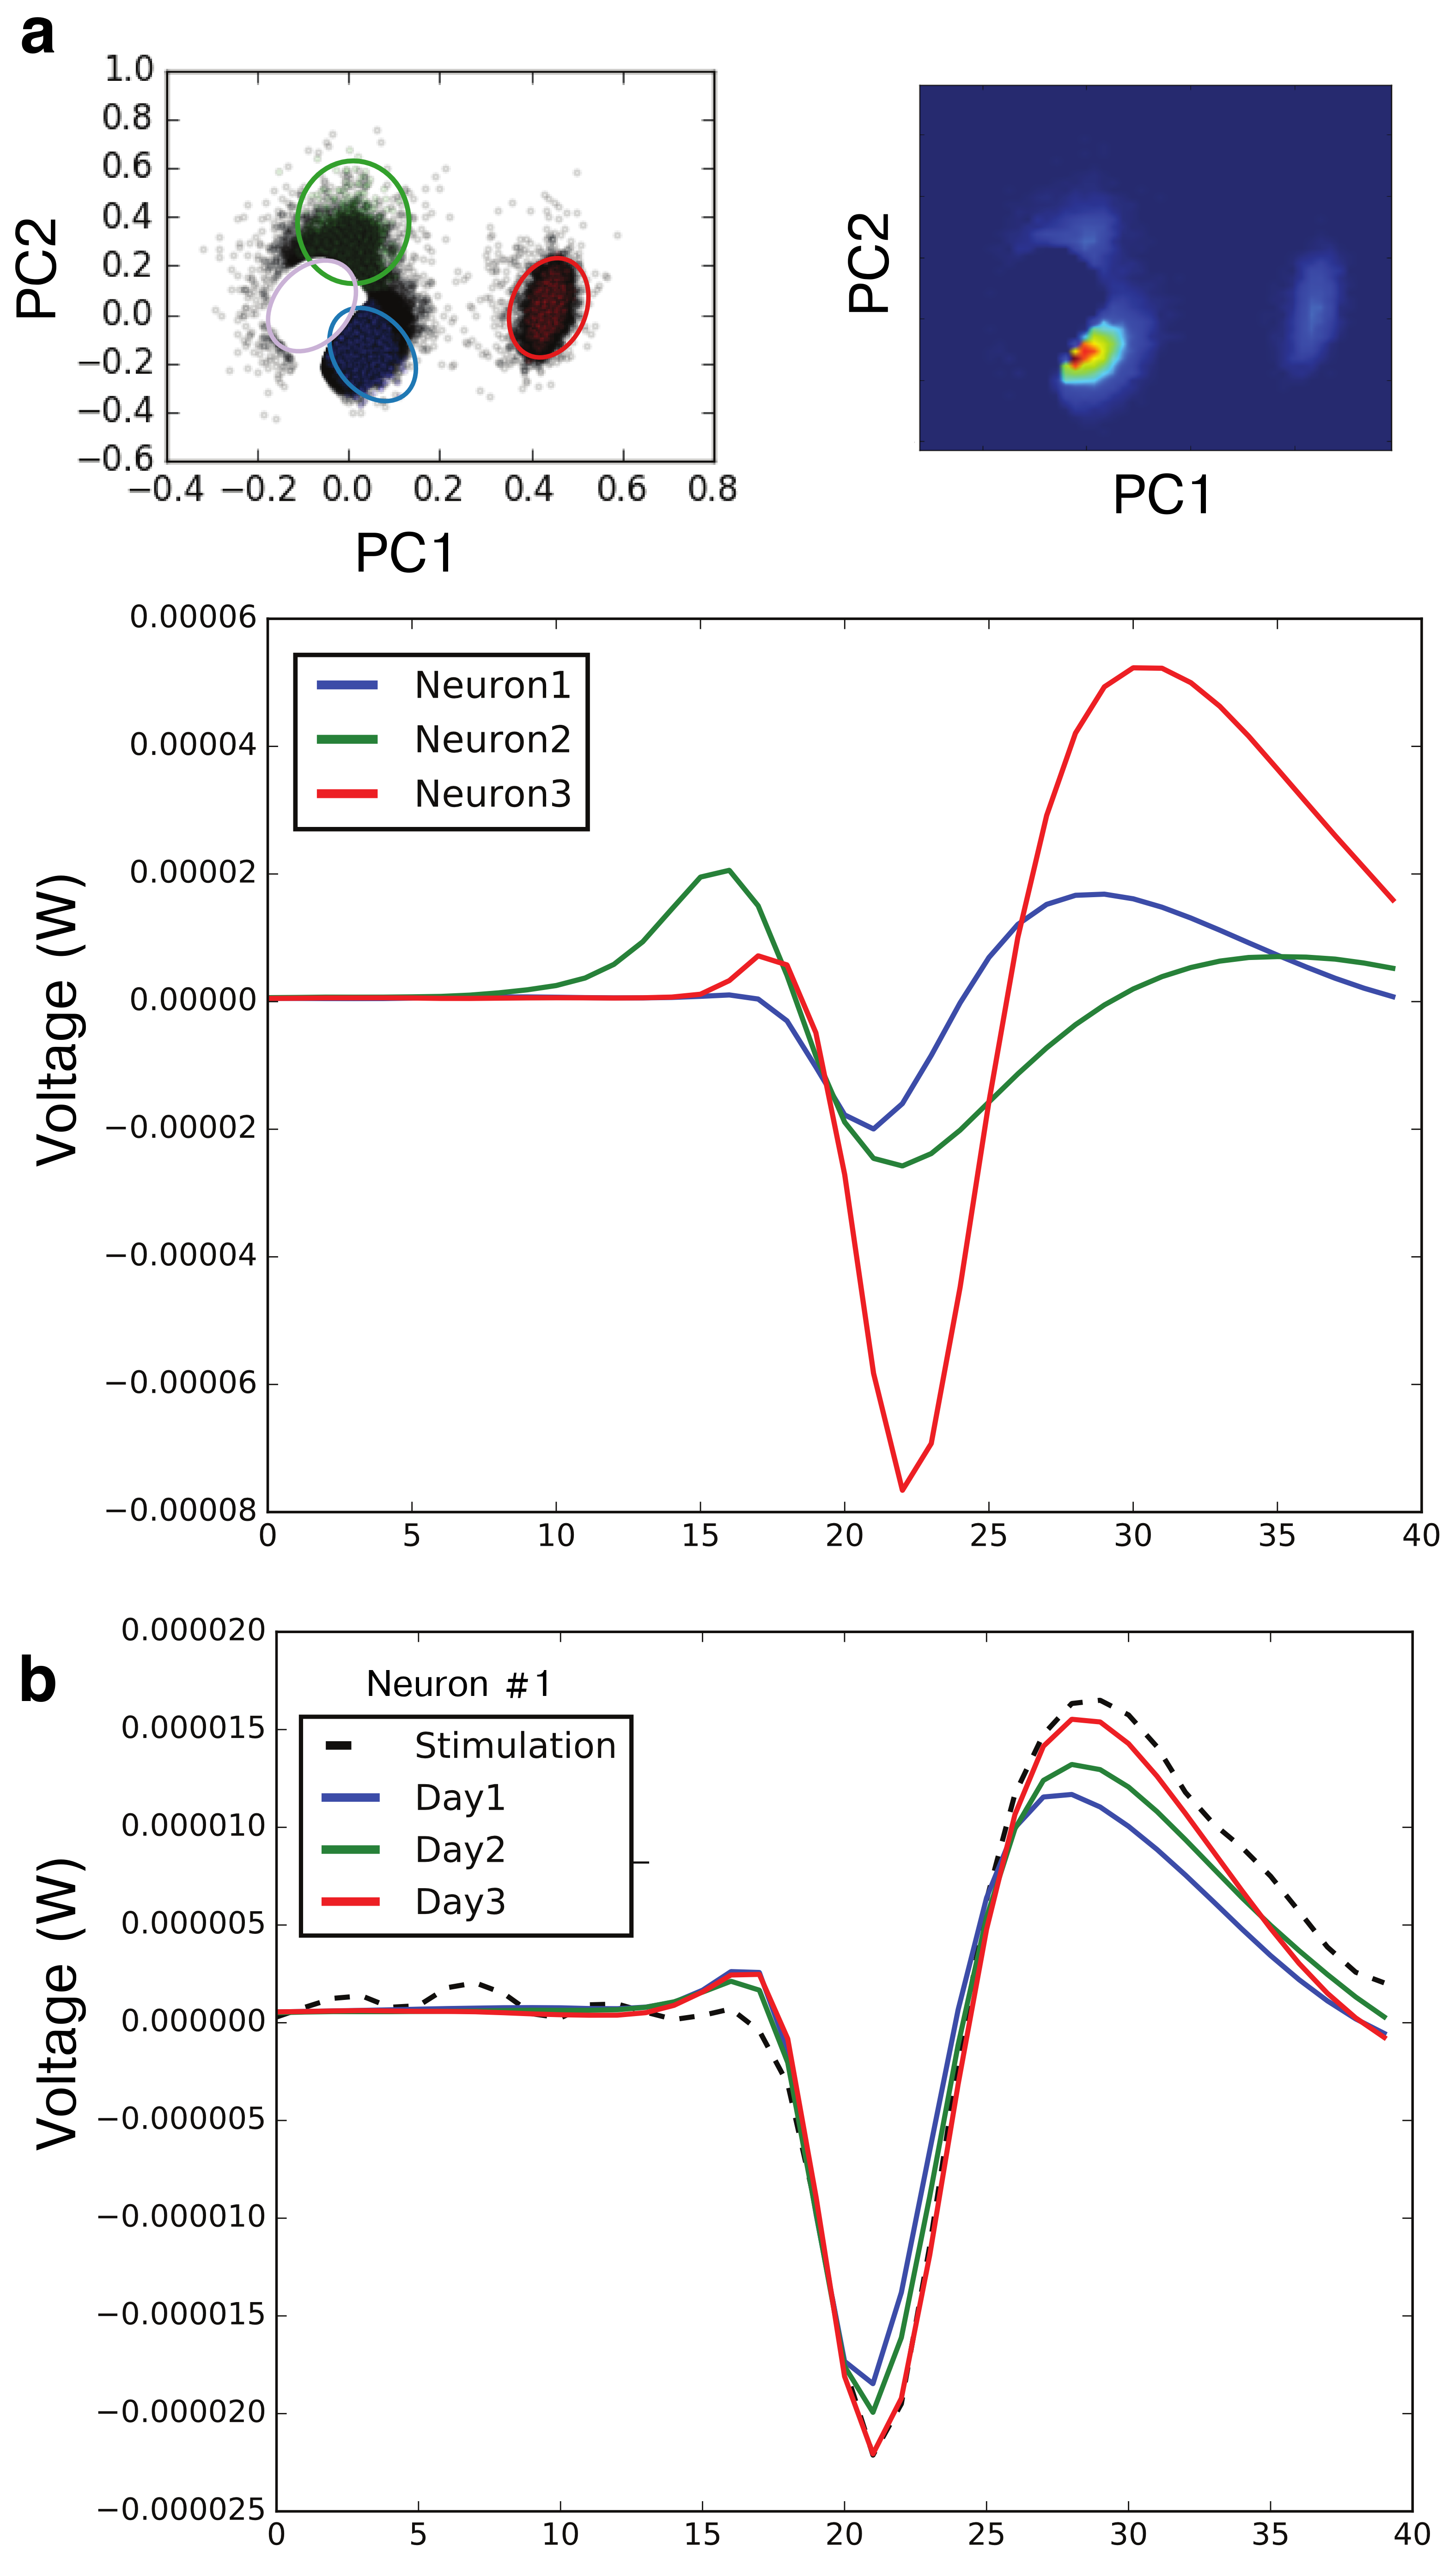
\includegraphics[width=3.5in]{chap5/figures/SupplementaryFigure1.png}
    \end{center}
    \caption{\label{fig:cms1} Spontaneous electrical firing from individual neurons can be reliably tracked across multiple days. We used a recursively applied PCA with Gaussian mixture model (GMM) clustering to discriminate firing from single SCN neurons across multiple days on multielectrode arrays before and during optogenetic stimulation. The automated analysis was performed blinded to the identity of the neuron (VIP or non-VIP). 
    (\textbf{a}) On this representative electrode, we identified 3 clusters (circled in top panel) and their corresponding average extracellular waveforms (bottom panel). The purple circle is the noise cluster which was identified and removed from analysis.
    (\textbf{b}) Neuron1 from the above analysis was identified as VIP-positive. The spike waveform during optogenetic stimulation (dashed line) correlated with the mean spontaneous activity waveforms recorded from each of the prior three days from the same electrode. 
    }
\end{figure}

\subsection*{Identifying spontaneous electrical activity of VIP neurons}
The aim of our first experiment was to identify relevant firing patterns and frequencies within the SCN, and to test the hypothesis that the subset of SCN neurons that express VIP exhibit also form a coherent electrophysiological class of neurons.
To characterize the firing of these neurons across multiple days, we recorded from high-density SCN neuronal cultures plated on multielectrode arrays (MEAs) for three days.
Extracellular recording from MEAs allowed the recording from dozens of individual neurons within an SCN culture, and prior studies have shown that neuronal activity in high-density SCN cultures corresponds well with recordings from SCN slices \textit{in vitro} and the intact SCN \textit{in vivo}.
As described in the methods, channelrhodopsin-2 (ChR2) was expressed solely in VIP neurons by crossing a floxed-ChR2 mouse line with a VIPCre mouse line.
Following the recording of spontaneous electrical activity, each culture received optogenetic stimulation, so that, by identifying which neurons respond to stimulation, we were able to retroactively classify neuronal identity by VIP content.
The schematic in Figure \ref{fig:cm1}a shows the experimental procedure for obtaining multiday recordings from MEAs containing VIP and nonVIP neurons.
Figure \ref{fig:cm1}b demonstrates the method for identifying VIP neurons retroactively.
The interspike interval histograms for a VIP neuron and a nonVIP neuron during a 4 Hz stimulus demonstrate that the VIP neuron responded by firing precisely in response to the stimulation pattern.
To further confirm that VIP neurons responded by firing synchronously, we cross-correlated spike times between pairs of SCN neurons (Figure \ref{fig:cm1}c).
As expected, only VIP neurons fired synchronously (with no lag) in response to optogenetic stimulation.
Furthermore, some nonVIP neurons responded with reductions in firing for approximately 10-20 ms following each stimulation, consistent with inhibitory signaling from VIP neurons.

Using this information, we retroactively classified the three prior days of spontaneous activity as VIP or nonVIP and in total, 8 MEAs resulted in multiday recordings from 40 VIP and 543 nonVIP SCN neurons.
Prior studies have relied on brief 1-30 min snapshots of VIP neuron firing, and reached opposing conclusions as to whether VIP neuron firing is circadian \cite{Fan2015, Hermanstyne2016}.
By tracking VIP neurons continuously across multiple days, we found that the majority ($81.5\pm4.0$\%, mean $\pm$ SEM, Figure \ref{fig:cm1}d-e) of VIP neurons in each culture were circadian, i.e.\ met the criteria for circadian oscillation as described in the methods.
In contrast, about half ($51.7\pm8.5$\%, mean $\pm$ SEM) of nonVIP neurons were circadian.

We performed additional experiments to test our assumptions that VIP neurons selectively and consistently responded to ChR2 stimulation.
First, we tested if ChR2 stimulation reliably triggered responses in ChR2 neurons by identifying VIPChR2 neurons via yEFP expression and using a whole-cell patch clamp recording technique (Figure \ref{fig:cms2}).
We found that only VIPChR2 neurons increased their firing rate to match that of the stimulus, and that these neurons reliably responded for frequencies between 2 and 15 Hz.
Next, we used a post-stimulus time histogram (PSTH, Figure \ref{fig:cms3}) to validate that these responded occurred within 5 ms of the stimulus.
Together, these results demonstrate a highly reliable optogenetic system for triggering firing of solely VIP neurons.
\begin{figure}[!p]
    \caption{\label{fig:cm1} 
    Characterizing multiday spontaneous firing activity of identified VIP SCN neurons within a multielectrode array culture.
    (\textbf{a}) SCN neurons were categorized as VIP-positive (VIP) or –negative (non-VIP) by optically tagging VIP neurons using optogenetic stimulation after 3 days of spontaneous activity recording.  Multiday firing was sorted from 583 SCN neurons identified on 8 multielectrode arrays plated and cultured for 3 weeks from VIPChR2 mice. Raster plots of five representative SCN neurons show how their spike times over one minute differed in mean rate and pattern. 
    (\textbf{b}) The inter-spike interval histograms during optogenetic stimulation illustrate how a representative VIP (top) neuron fired at the stimulation frequency (4 Hz) with a precision of <10ms (top right inset) and a non-VIP neuron (bottom) fired in a ChR2-independent pattern. 
    (\textbf{c}) To further characterize the evoked firing of VIP neurons, we cross-correlated spike times between concurrently recorded SCN neurons during optogenetic stimulation. A VIP reference neuron (top left panel) fired synchronously with 3 other representative VIP (top panels), but not 4 representative non-VIP neurons (bottom panels). Note that some non-VIP neurons (\#2 and \#3) decreased their firing following stimulation of VIP neurons, indicative of postsynaptic inhibition. 
    (\textbf{d}) Four representative VIP (top) and non-VIP (bottom panels) SCN neurons showing circadian firing patterns over the three days of recording. 
    (\textbf{e}) A greater fraction of VIP neurons were circadian ($81.6 \pm 4.7$\%) compared to non-VIP neurons ($51.7 \pm 8.5$\%, Chi-squared test **$P< 0.00001$). 
    (\textbf{f}) eYFP fluorescence (green) reveals the subset of SCN neurons expressing ChR2 near 4/60 electrodes.
    }
\end{figure}
\begin{figure}[p]
    \begin{center}
        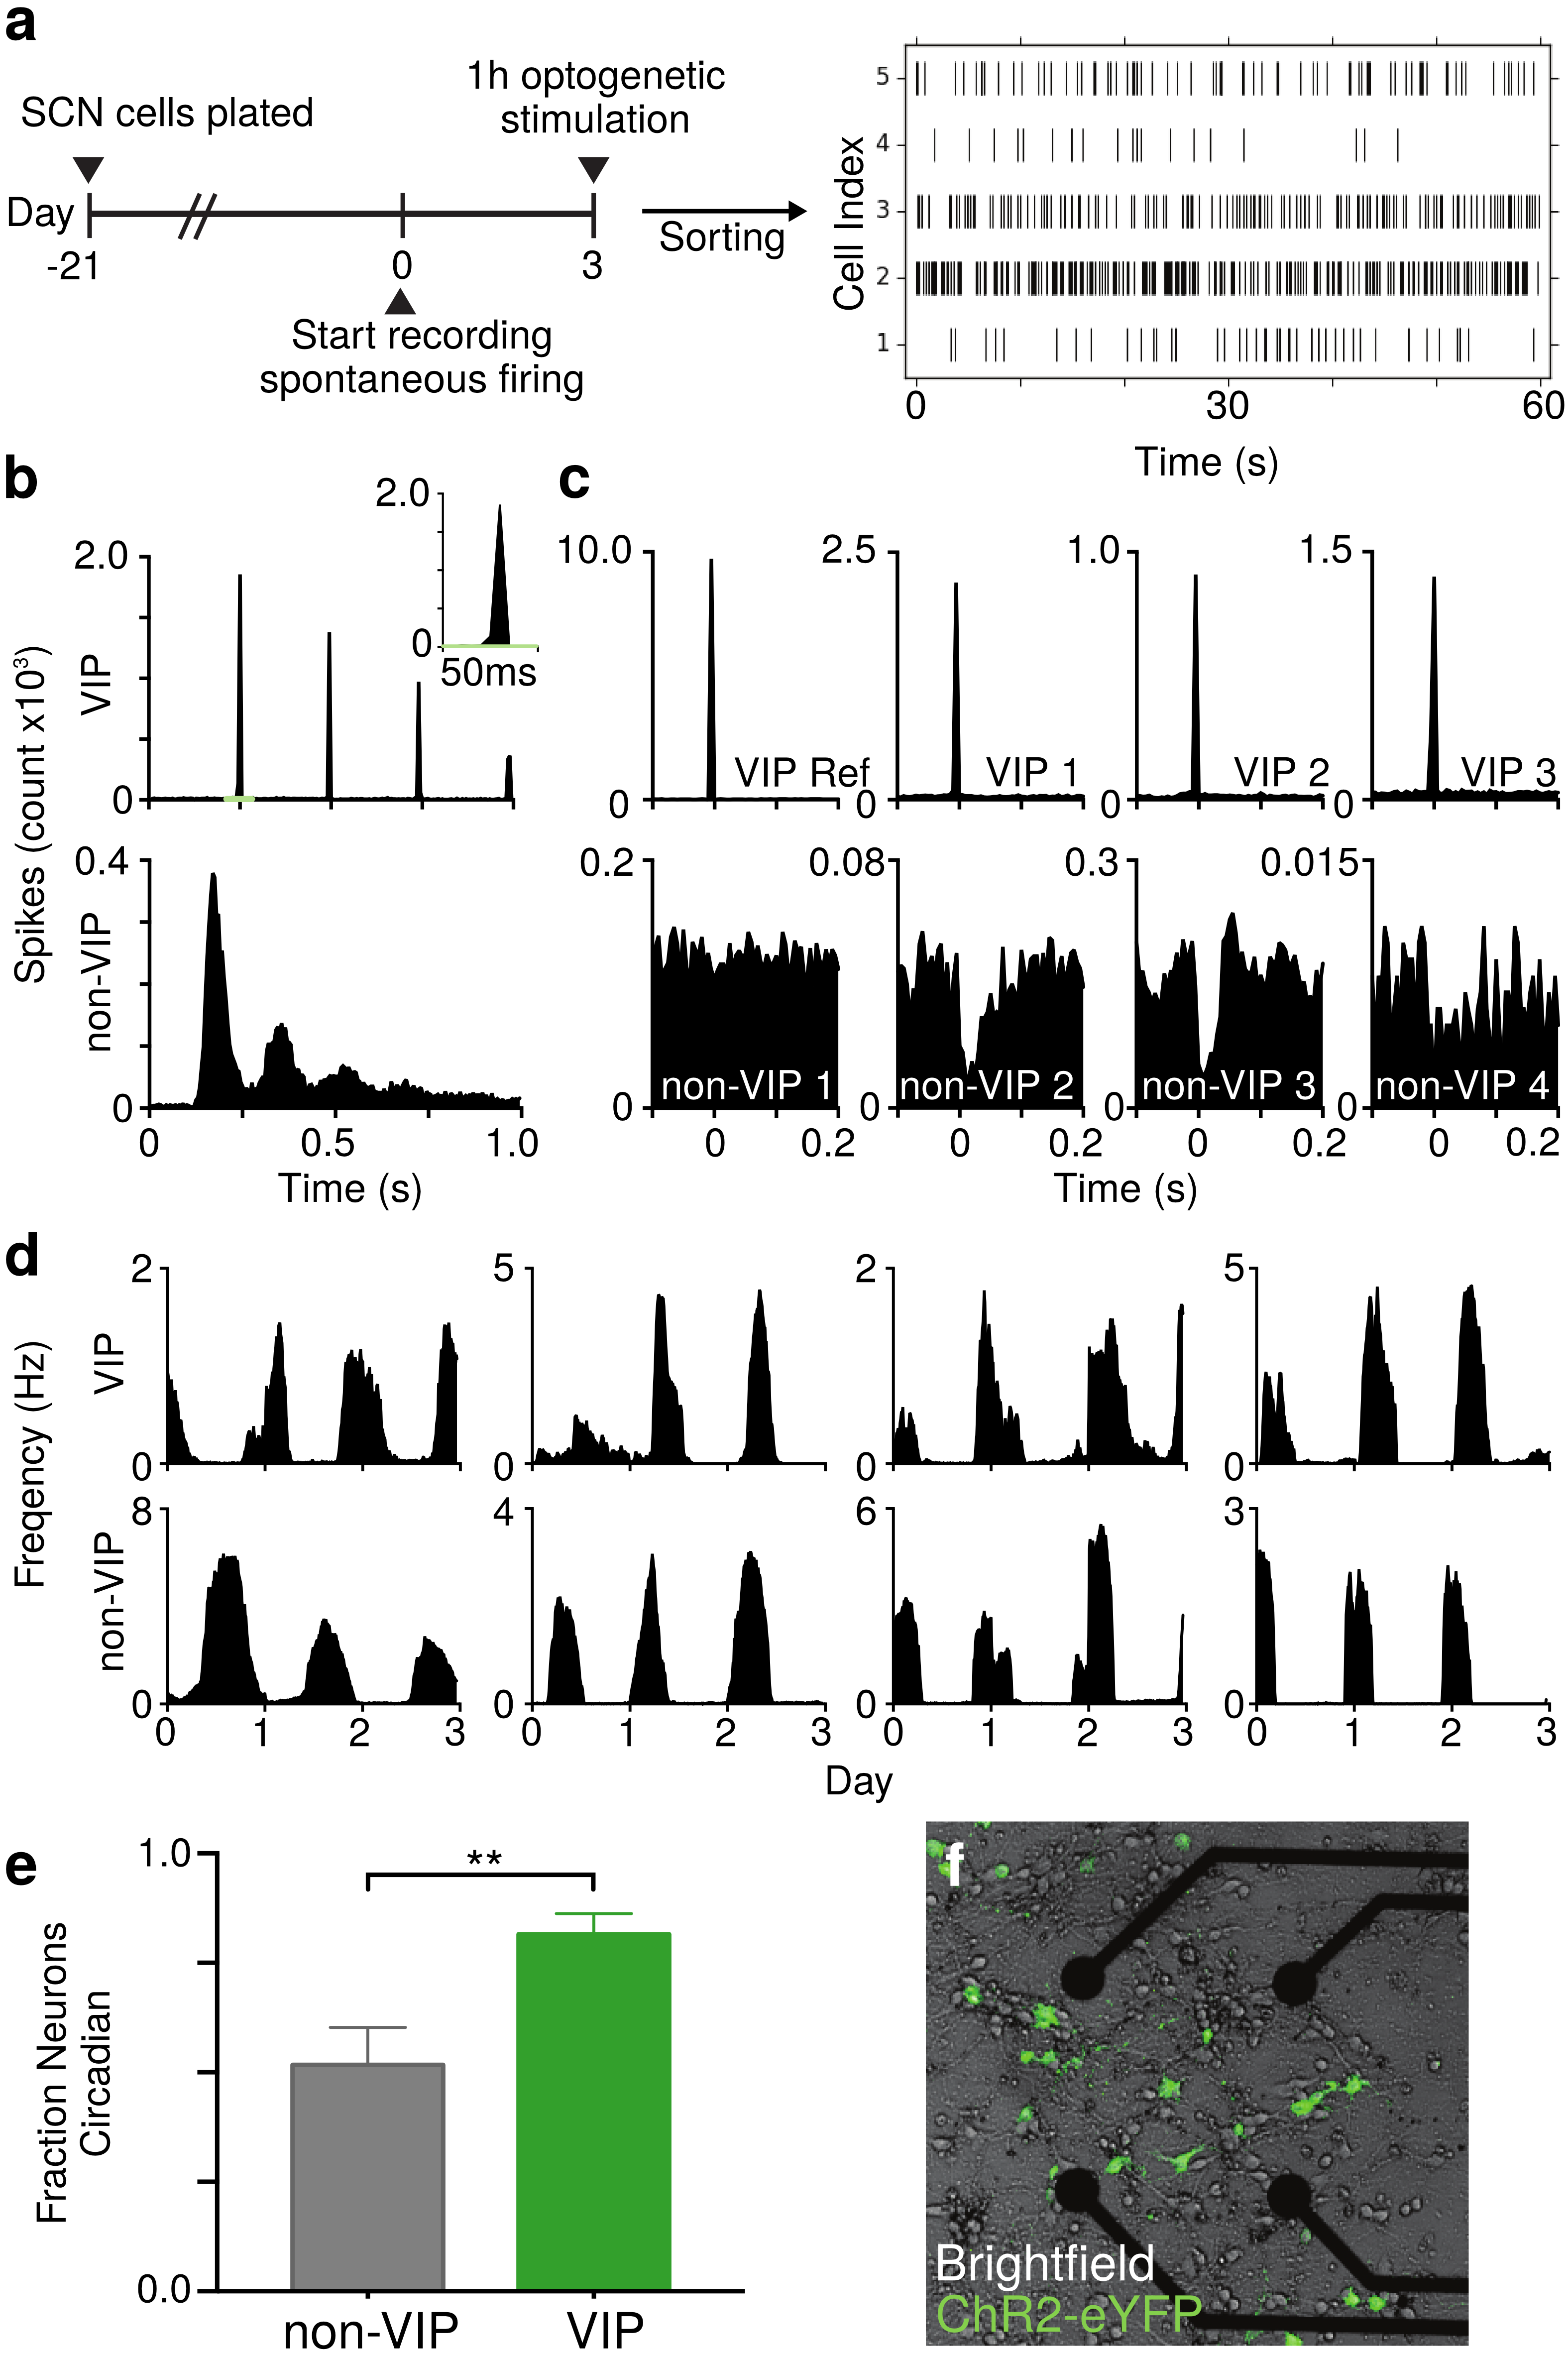
\includegraphics[width=4.5in]{chap5/figures/Figure1.png}
    \end{center}
\contcaption{(Continued.)}
\end{figure}
\clearpage
\begin{figure}[p]
    \begin{center}
        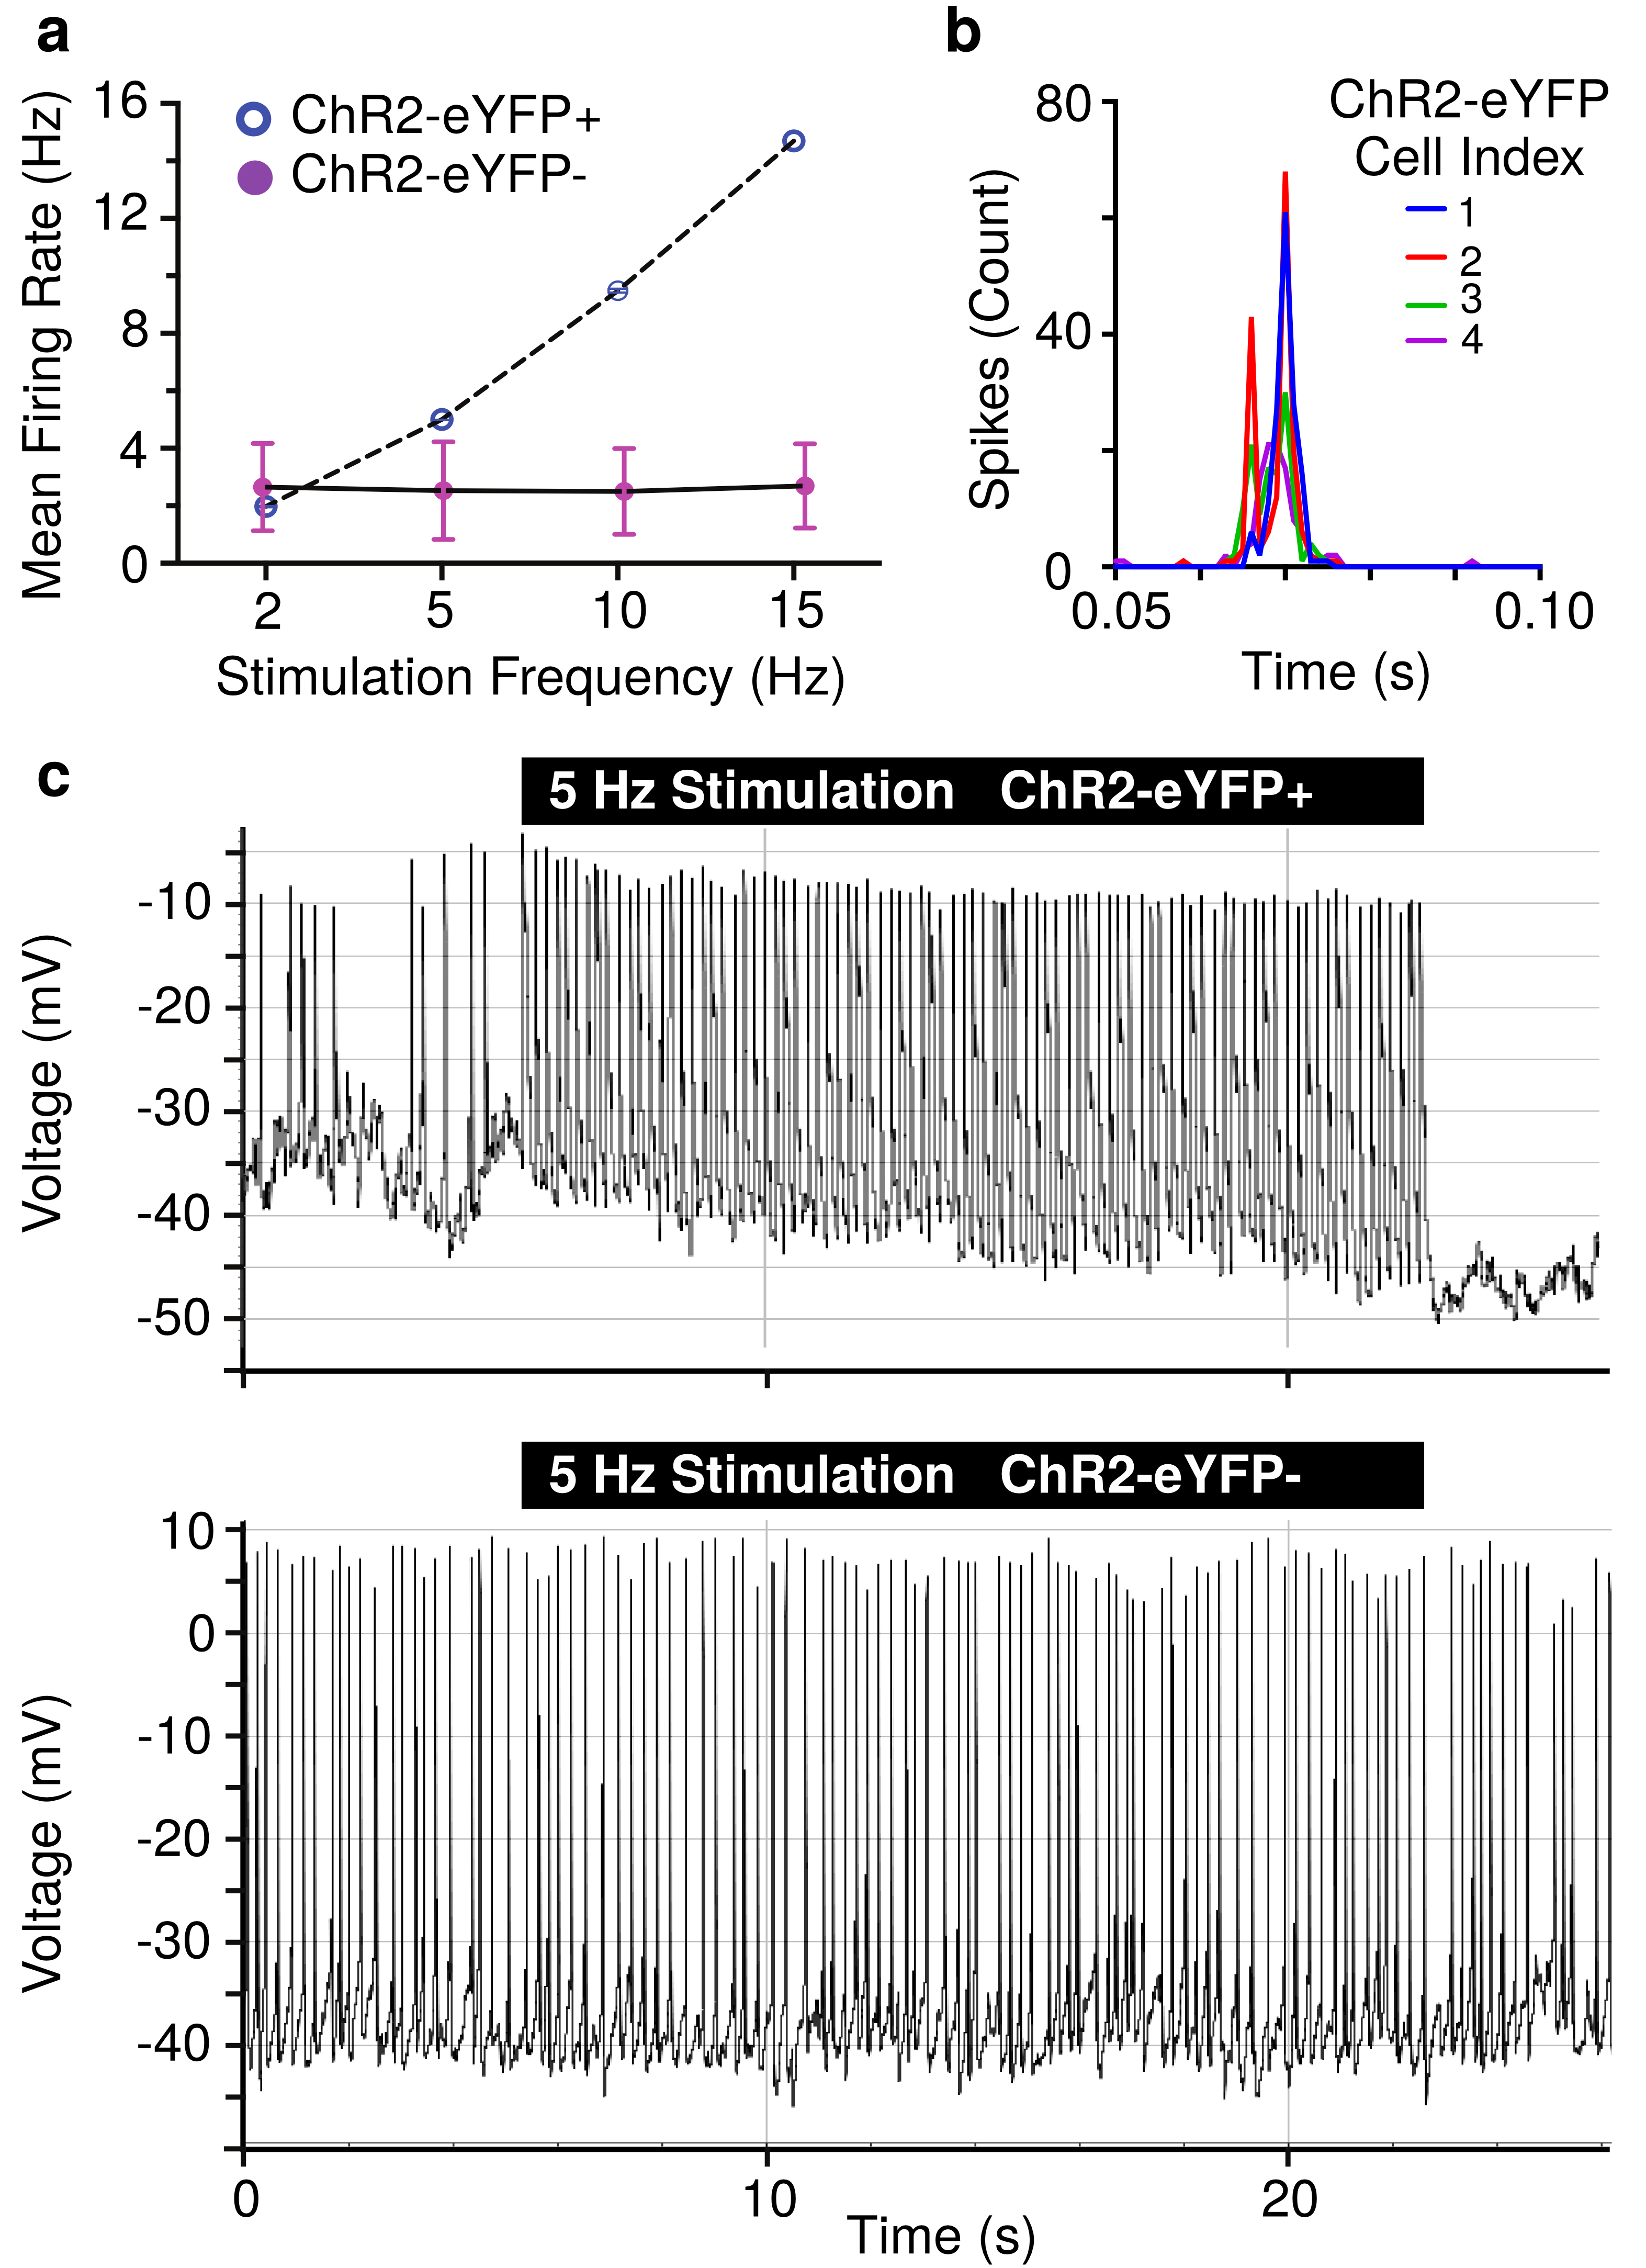
\includegraphics[width=3.5in]{chap5/figures/SupplementaryFigure2.png}
    \end{center}
    \caption{\label{fig:cms2} 
    Only ChR2 positive SCN neurons increase firing in response to optogenetic stimulation. 
    (\textbf{a}) Using whole-cell patch clamp, we recorded from neurons within VIPChR2 SCN slices while stimulating at 2, 5, 10, or 15 Hz. ChR2-eYFP positive neurons ($n = 5$) matched their firing to the stimulation frequency, while ChR2-eYFP negative neurons ($n = 5$) in the same SCN slice did not. 
    (\textbf{b}) ChR2-eYFP positive neurons followed the stimulation frequency within 10 ms as revealed by the interspike interval histogram (15 Hz stimulation, $n = 4$ neurons). 
    (\textbf{c}) Representative traces show a ChR2-eYFP positive neuron that increased its firing rate in response to 5 Hz stimulation, while ChR2-eYFP negative firing did not change. These results indicate that the presence of ChR2 is necessary for light-evoked increases in firing. 
    }
\end{figure}

\begin{figure}[p]
    \begin{center}
        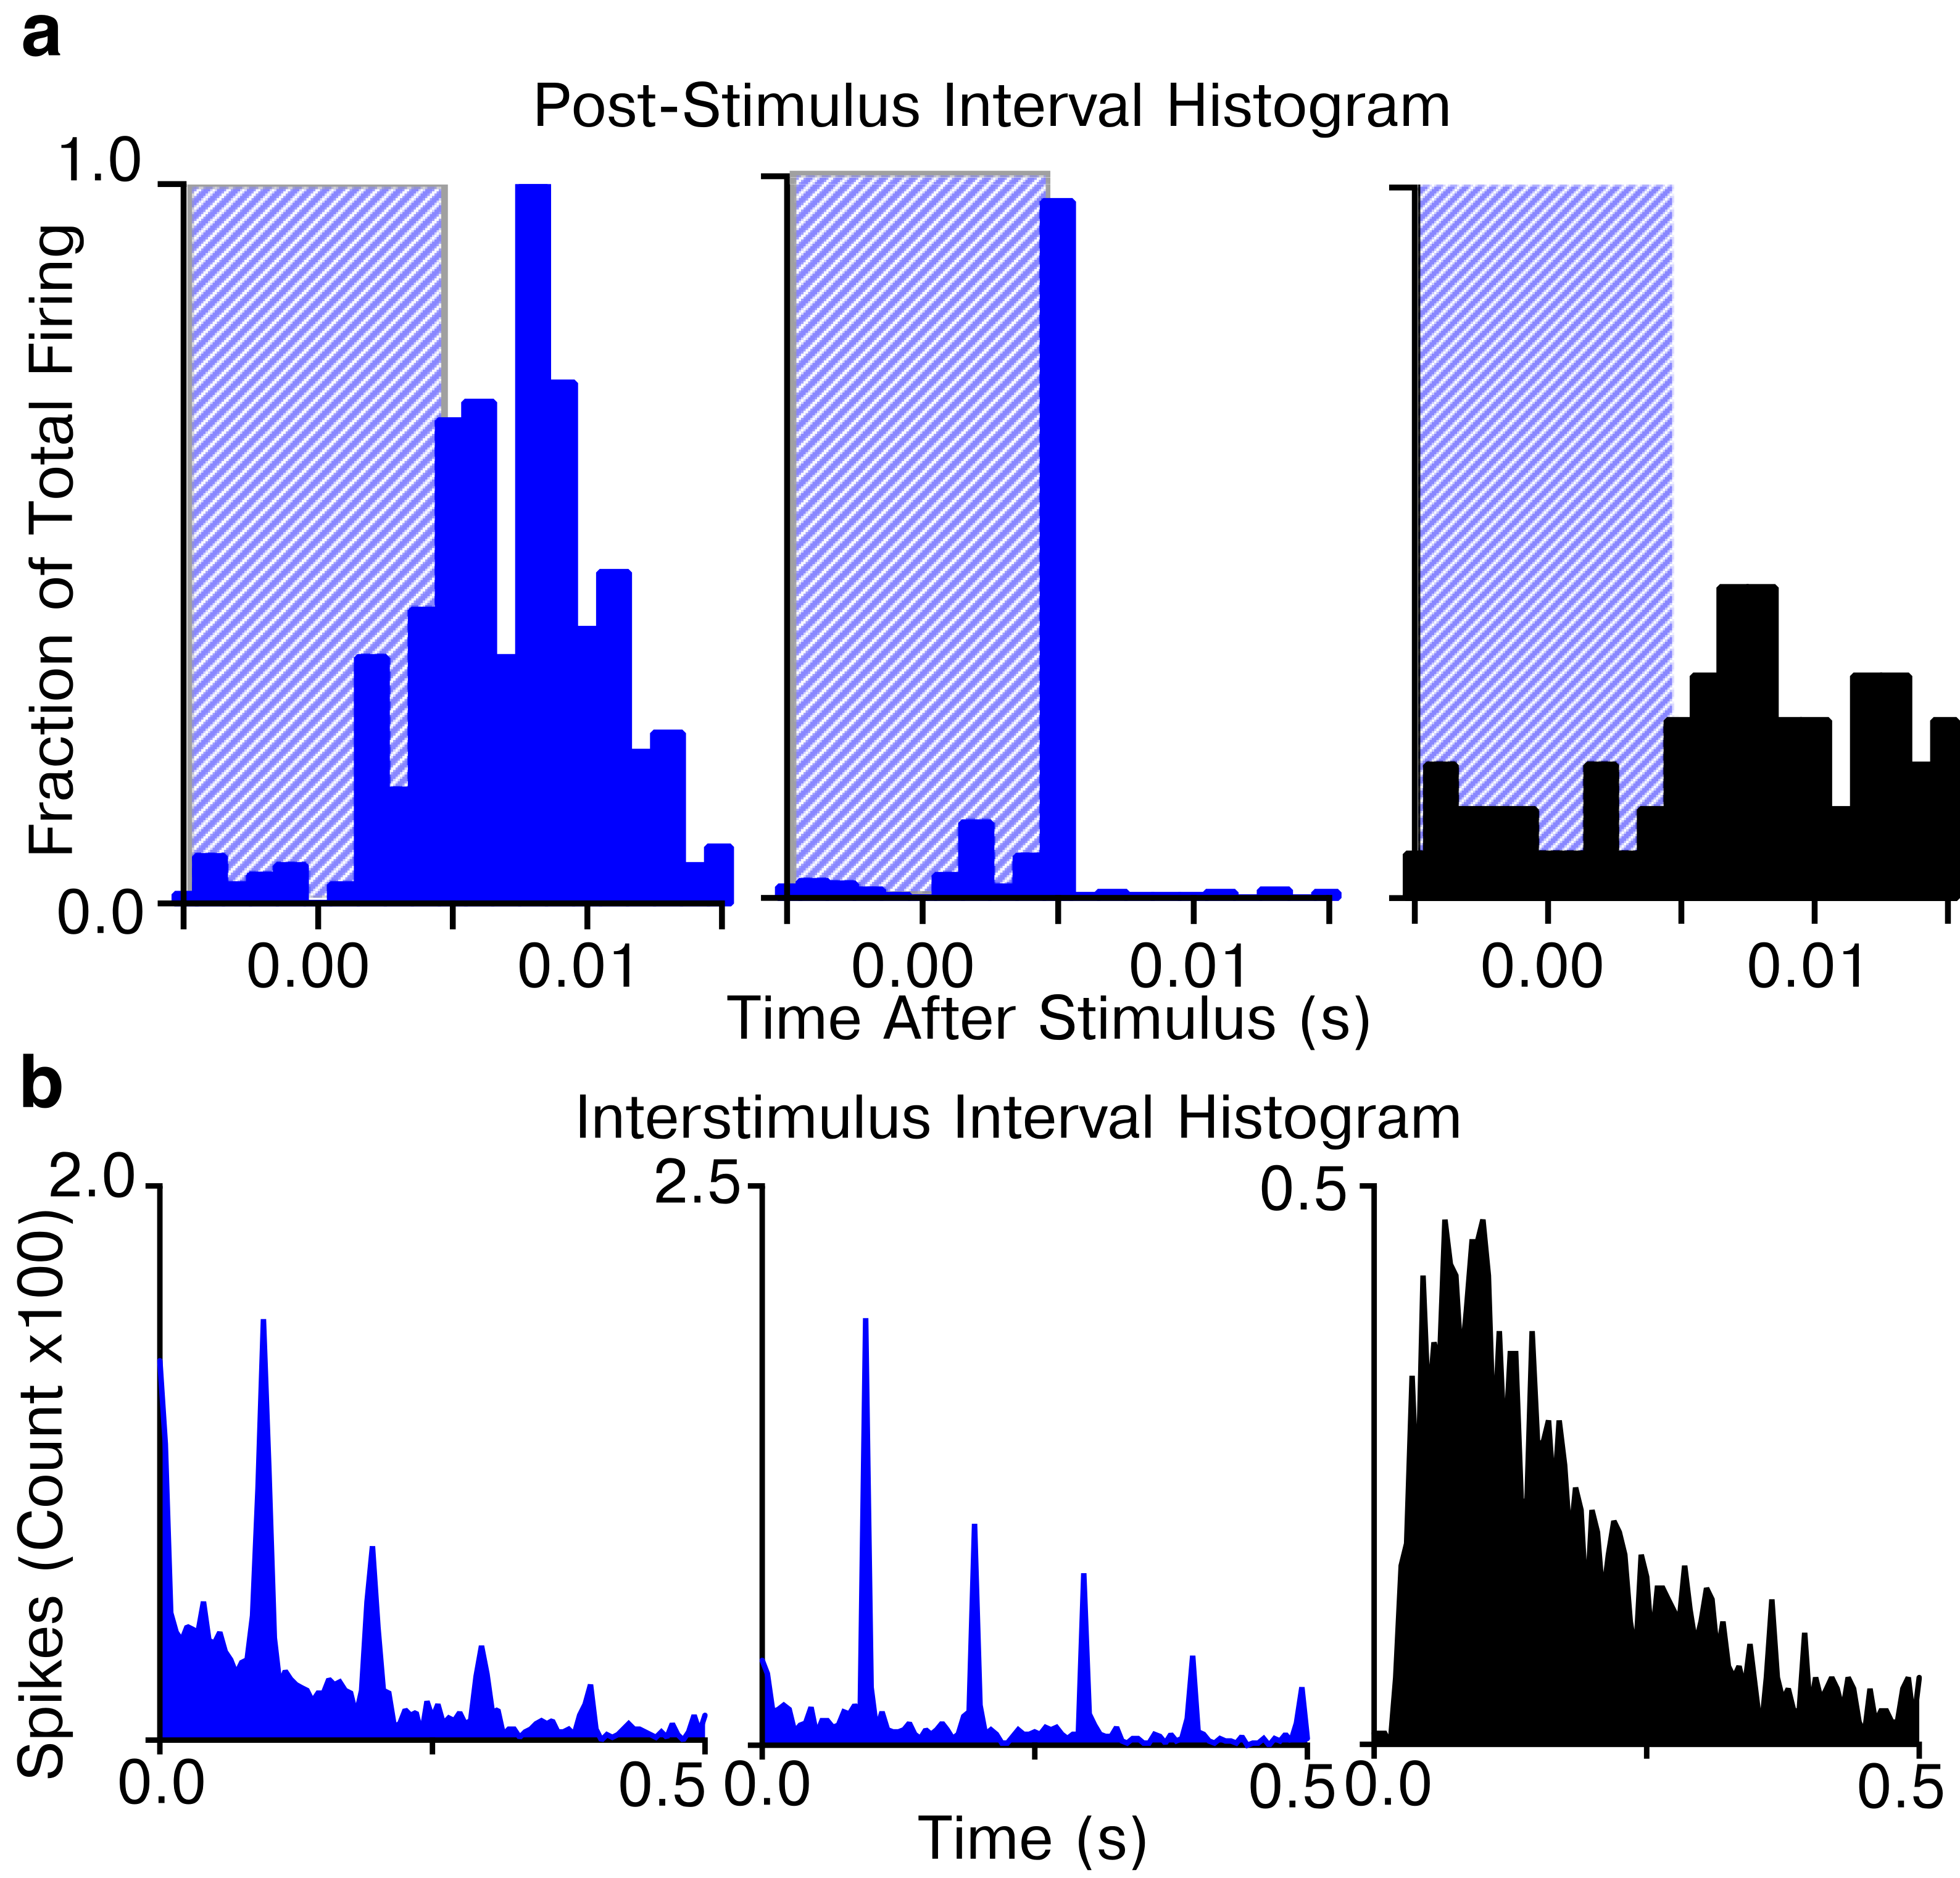
\includegraphics[width=3.5in]{chap5/figures/SupplementaryFigure3.png}
    \end{center}
    \caption{\label{fig:cms3} 
        VIPChR2 neurons fire within 10 ms of  stimulation.
    (\textbf{a}) The post-stimulus histogram (PSTH) of SCN neuronal firing following a 10 ms laser flash (blue box) showed that 100\% of neurons identified as VIPergic (blue) fired reliably within 10ms of the stimulation, while non-VIP neurons (black) did not respond to the flashes. 
    (\textbf{b}) Corresponding ISIH for two VIP (blue) and one non-VIP (black) neurons during 10 Hz stimulation. The VIP neuron fired at 0.1 s intervals whereas the non-VIP neuron (black) did not. Thus, the ISIH or the PSTH accurately identified VIP neurons on multielectrode arrays.
    }
\end{figure}


\subsection*{VIP neurons exhibit multiple distinct firing patterns}

Prior studies have focused on circadian variations in mean firing rates through binning electrical activity into seconds-to-minutes long epochs.
However, it is millisecond-to-second firing patterns and short-term firing frequency that have been implicated in neurotransmitter release probability and changes in calcium transients \cite{Tsodyks1997, Neher2008}.
Therefore, we analyzed the resulting circadian neurons ($n=268$ nonVIP and $n=33$ VIP) to characterize the physiologically relevant instantaneous firing frequencies.

Using the spike timing (or interspike interval histogram (ISIH) of the entire recording) and a hierarchical clustering, we found three distinct classes of firing pattern, similar to those observed in \cite{Pennartz1998}.
These classes were tonic (i.e.\ characterized by a highly regular timing between spikes), irregular (i.e.\ characterized by a wide variability in spacing between spikes), and bursting (i.e., characterized by infrequent bursts of several spikes at frequencies in excess of 50 Hz).
Contrary to our expectation, VIP neurons were classified into multiple categories of firing pattern, indicating that they are an electrophysiologically heterogeneous group of neurons.
This result is shown in Figure \ref{fig:cm2}a-b.
We note that our classification scheme does not indicate that, for example, an irregular neuron could never burst, but instead that irregular spiking represents the dominant mode of its electrical activity.
For each neuron, we then identified the dominant instantaneous firing rate (DIFF): the firing frequency associated with the peak of the ISI histogram (Figure \ref{fig:cm2}d).

Intriguingly, we did not observe day-to-day changes in neuronal firing class despite drastic changes in mean firing rate across the circadian day (Figure \ref{fig:cm2}e).
That is, a tonic neuron may be silent for its subjective night, but will resume tonic firing the next day with ISI corresponding to that of the previous day.
To determine if these patterns were consistent with \textit{in vivo} neuronal function, we analyzed the data from \cite{Hermanstyne2016} using an identical hierarchical clustering.
These VIP data were also classified as electrophysiologically heterogeneous, with clusters corresponding to the tonic and irregular clusters identified from MEA recordings.
Representative 60 s firing from each of the electrophysiological classes are shown in Figure \ref{fig:cms4}.
In sum, we found that VIP neurons, despite being a small subset of the SCN, are members of distinct and consistent electrophysiological classes and largely fire with tonic or irregular spike timing, at peak frequencies of approximately 2-10 Hz.
\clearpage
\begin{figure}[!p]
    \caption{\label{fig:cm2} 
    VIP-expressing SCN neurons exhibit tonic or irregular circadian firing patterns.
    (\textbf{a}) Hierarchical clustering sorts SCN neuron recordings from multielectrode arrays into one of three different daytime firing patterns: Tonic (TON), irregular (IRR) or bursting (BUR). Identification of VIP neurons (black lines) reveal that they are a heterogeneous class of neurons that exhibit either tonic or irregular firing. 
    (\textbf{b})  Representative interspike interval histograms (ISIH) for each identified class of neurons. The dominant instantaneous firing frequency (DIFF, black triangle) measures the most common firing interval for an individual neuron. 
    (\textbf{c}) The total ISIH for VIP and nonVIP neurons. 
    (\textbf{d}) Quantification of the DIFF from each class (n = the number of neurons recorded within each class; median interquartile range in Hz: TON VIP $5.3 \pm 2.8$, IRR VIP $3.9 \pm 3.7$, TON Non-VIP $6.2 \pm 3.6$, IRR Non-VIP $4.1 \pm 4.1$, BUR Non-VIP $101.0 \pm 73.6$). 
    (\textbf{e}) Short-term firing patterns were stable across multiple days shown by three representative SCN neurons. Note that the daily appearance of multiple bands during tonic firing corresponds to harmonics resulting from skipped spikes. 
    (\textbf{f}) Daytime firing VIP neurons recording using whole-cell patch clamp (data previously published in \cite{Hermanstyne2016}) similarly exhibit tonic or irregular firing. 
    (\textbf{g}) Representative ISIH from these neurons.
    (\textbf{h}) Dominant instantaneous firing rate was calculated for each neuron from the ISIH peak, and a boxplot of dominant frequency is shown for each neuron class (tonic/irregular). Observed DIFF fell predominantly between 2 Hz and 10 Hz (tonic VIP $4.5 \pm 1.4$ Hz; irregular VIP $2.8 \pm 1.4$ Hz; all values median $\pm$ interquartile range).
    }
\end{figure}
\begin{figure}[p]
    \begin{center}
        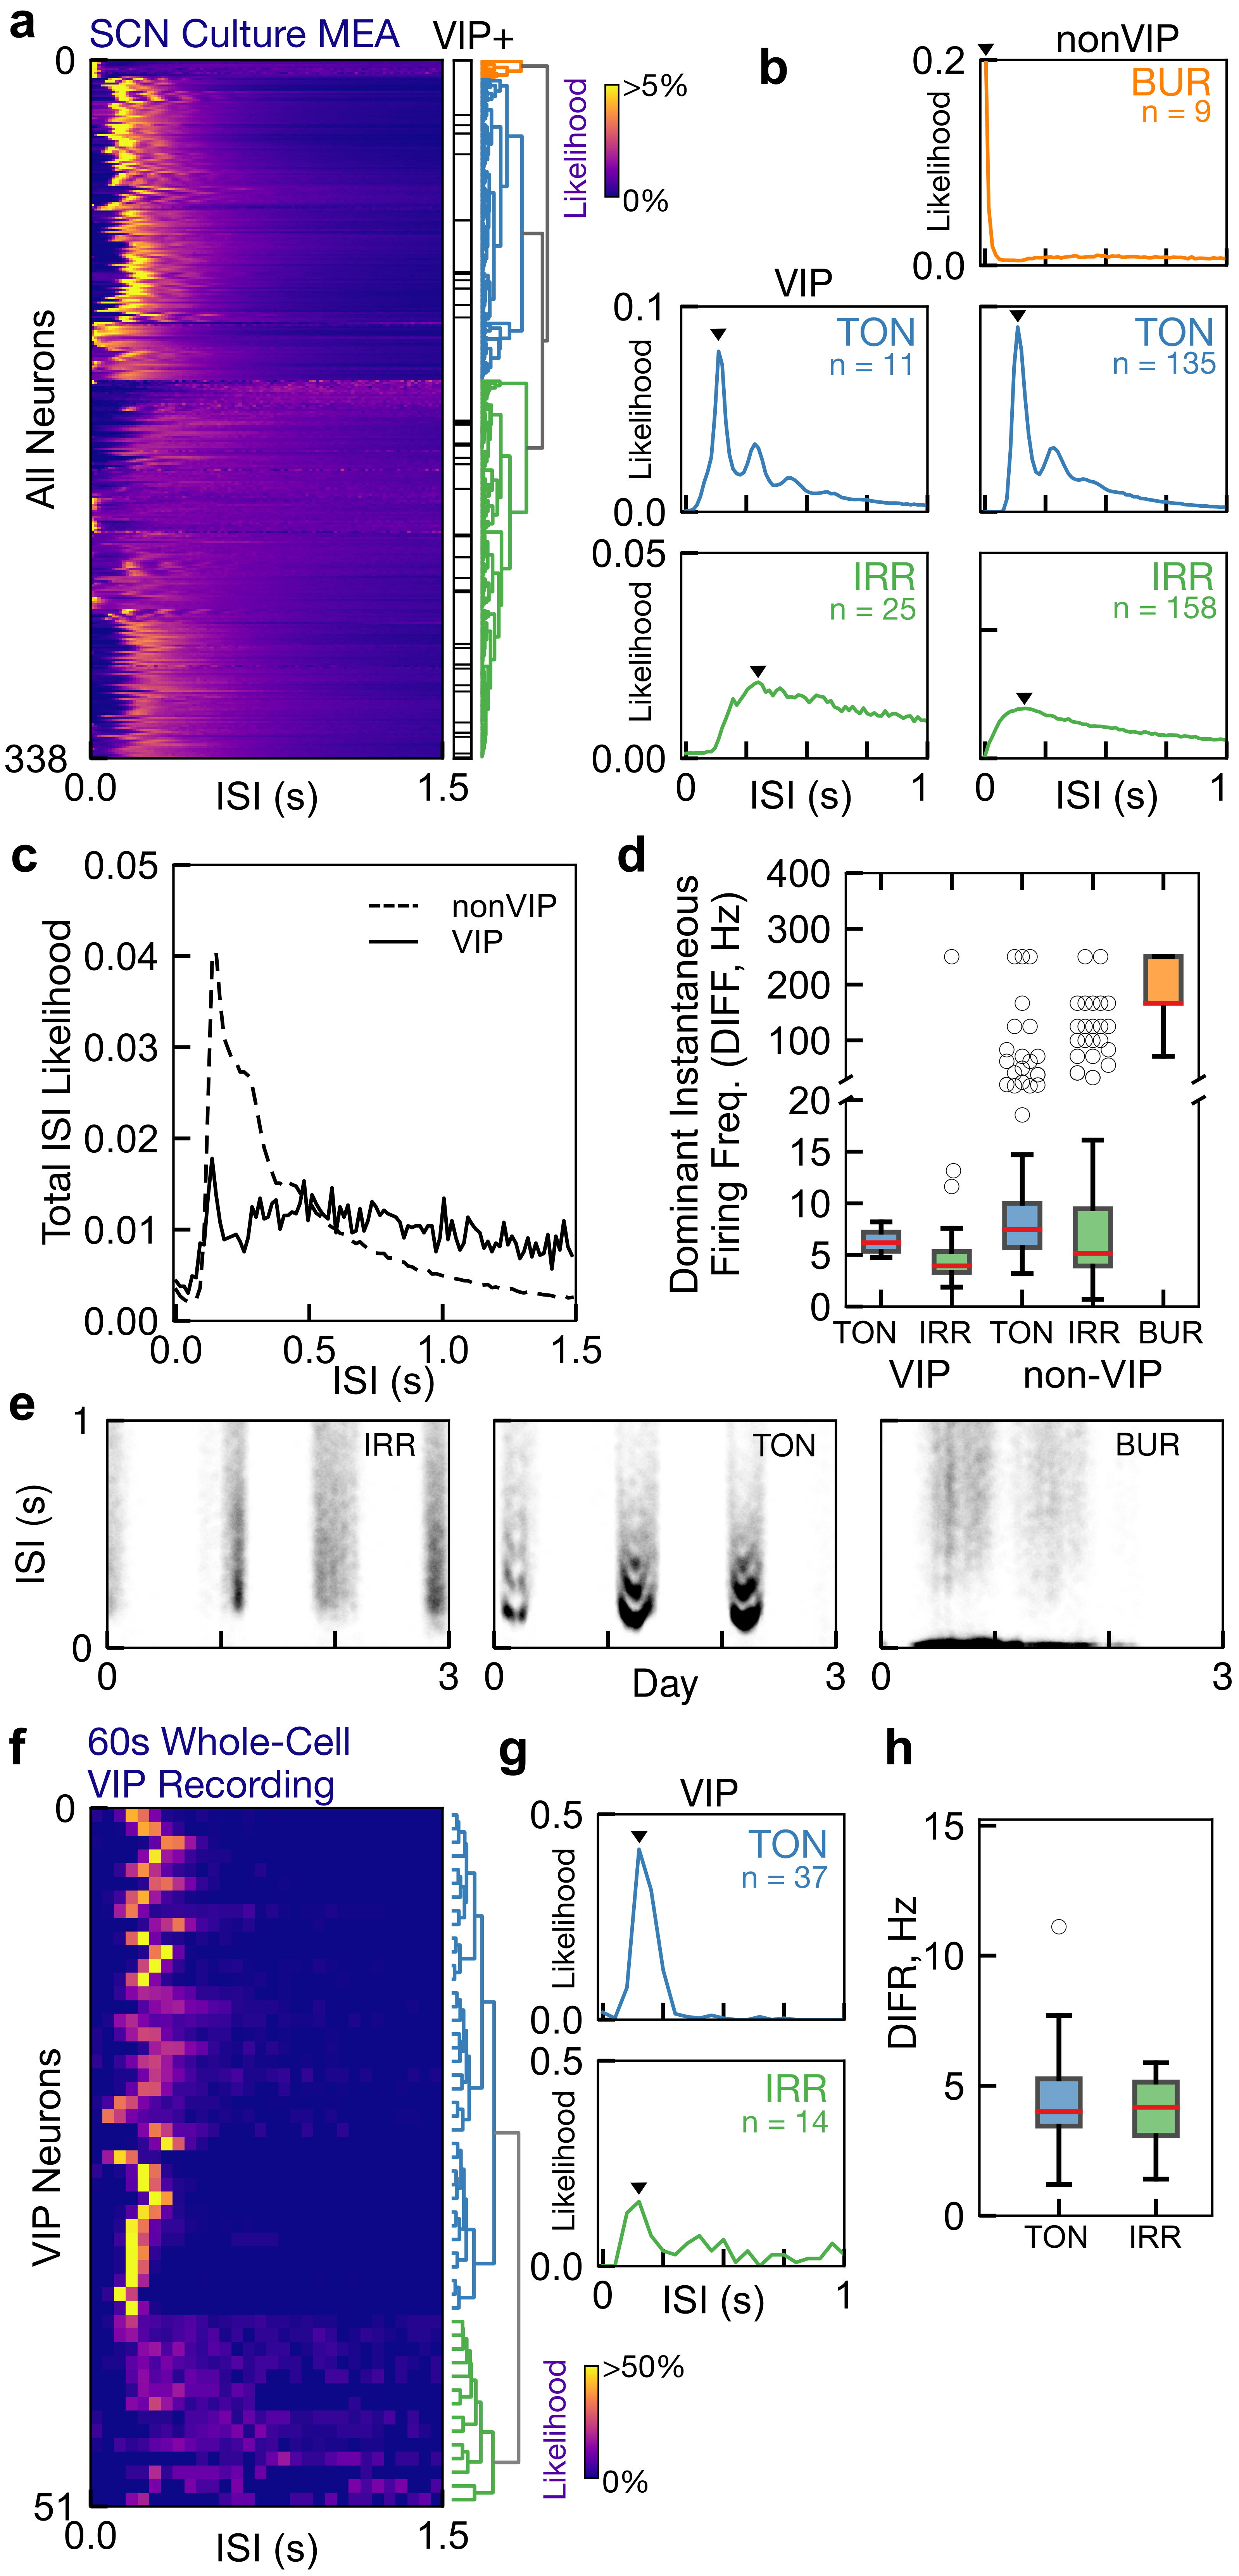
\includegraphics[width=3.5in]{chap5/figures/Figure2.png}
    \end{center}
\contcaption{(Continued.)}
\end{figure}
\clearpage
\begin{figure}[p]
    \begin{center}
        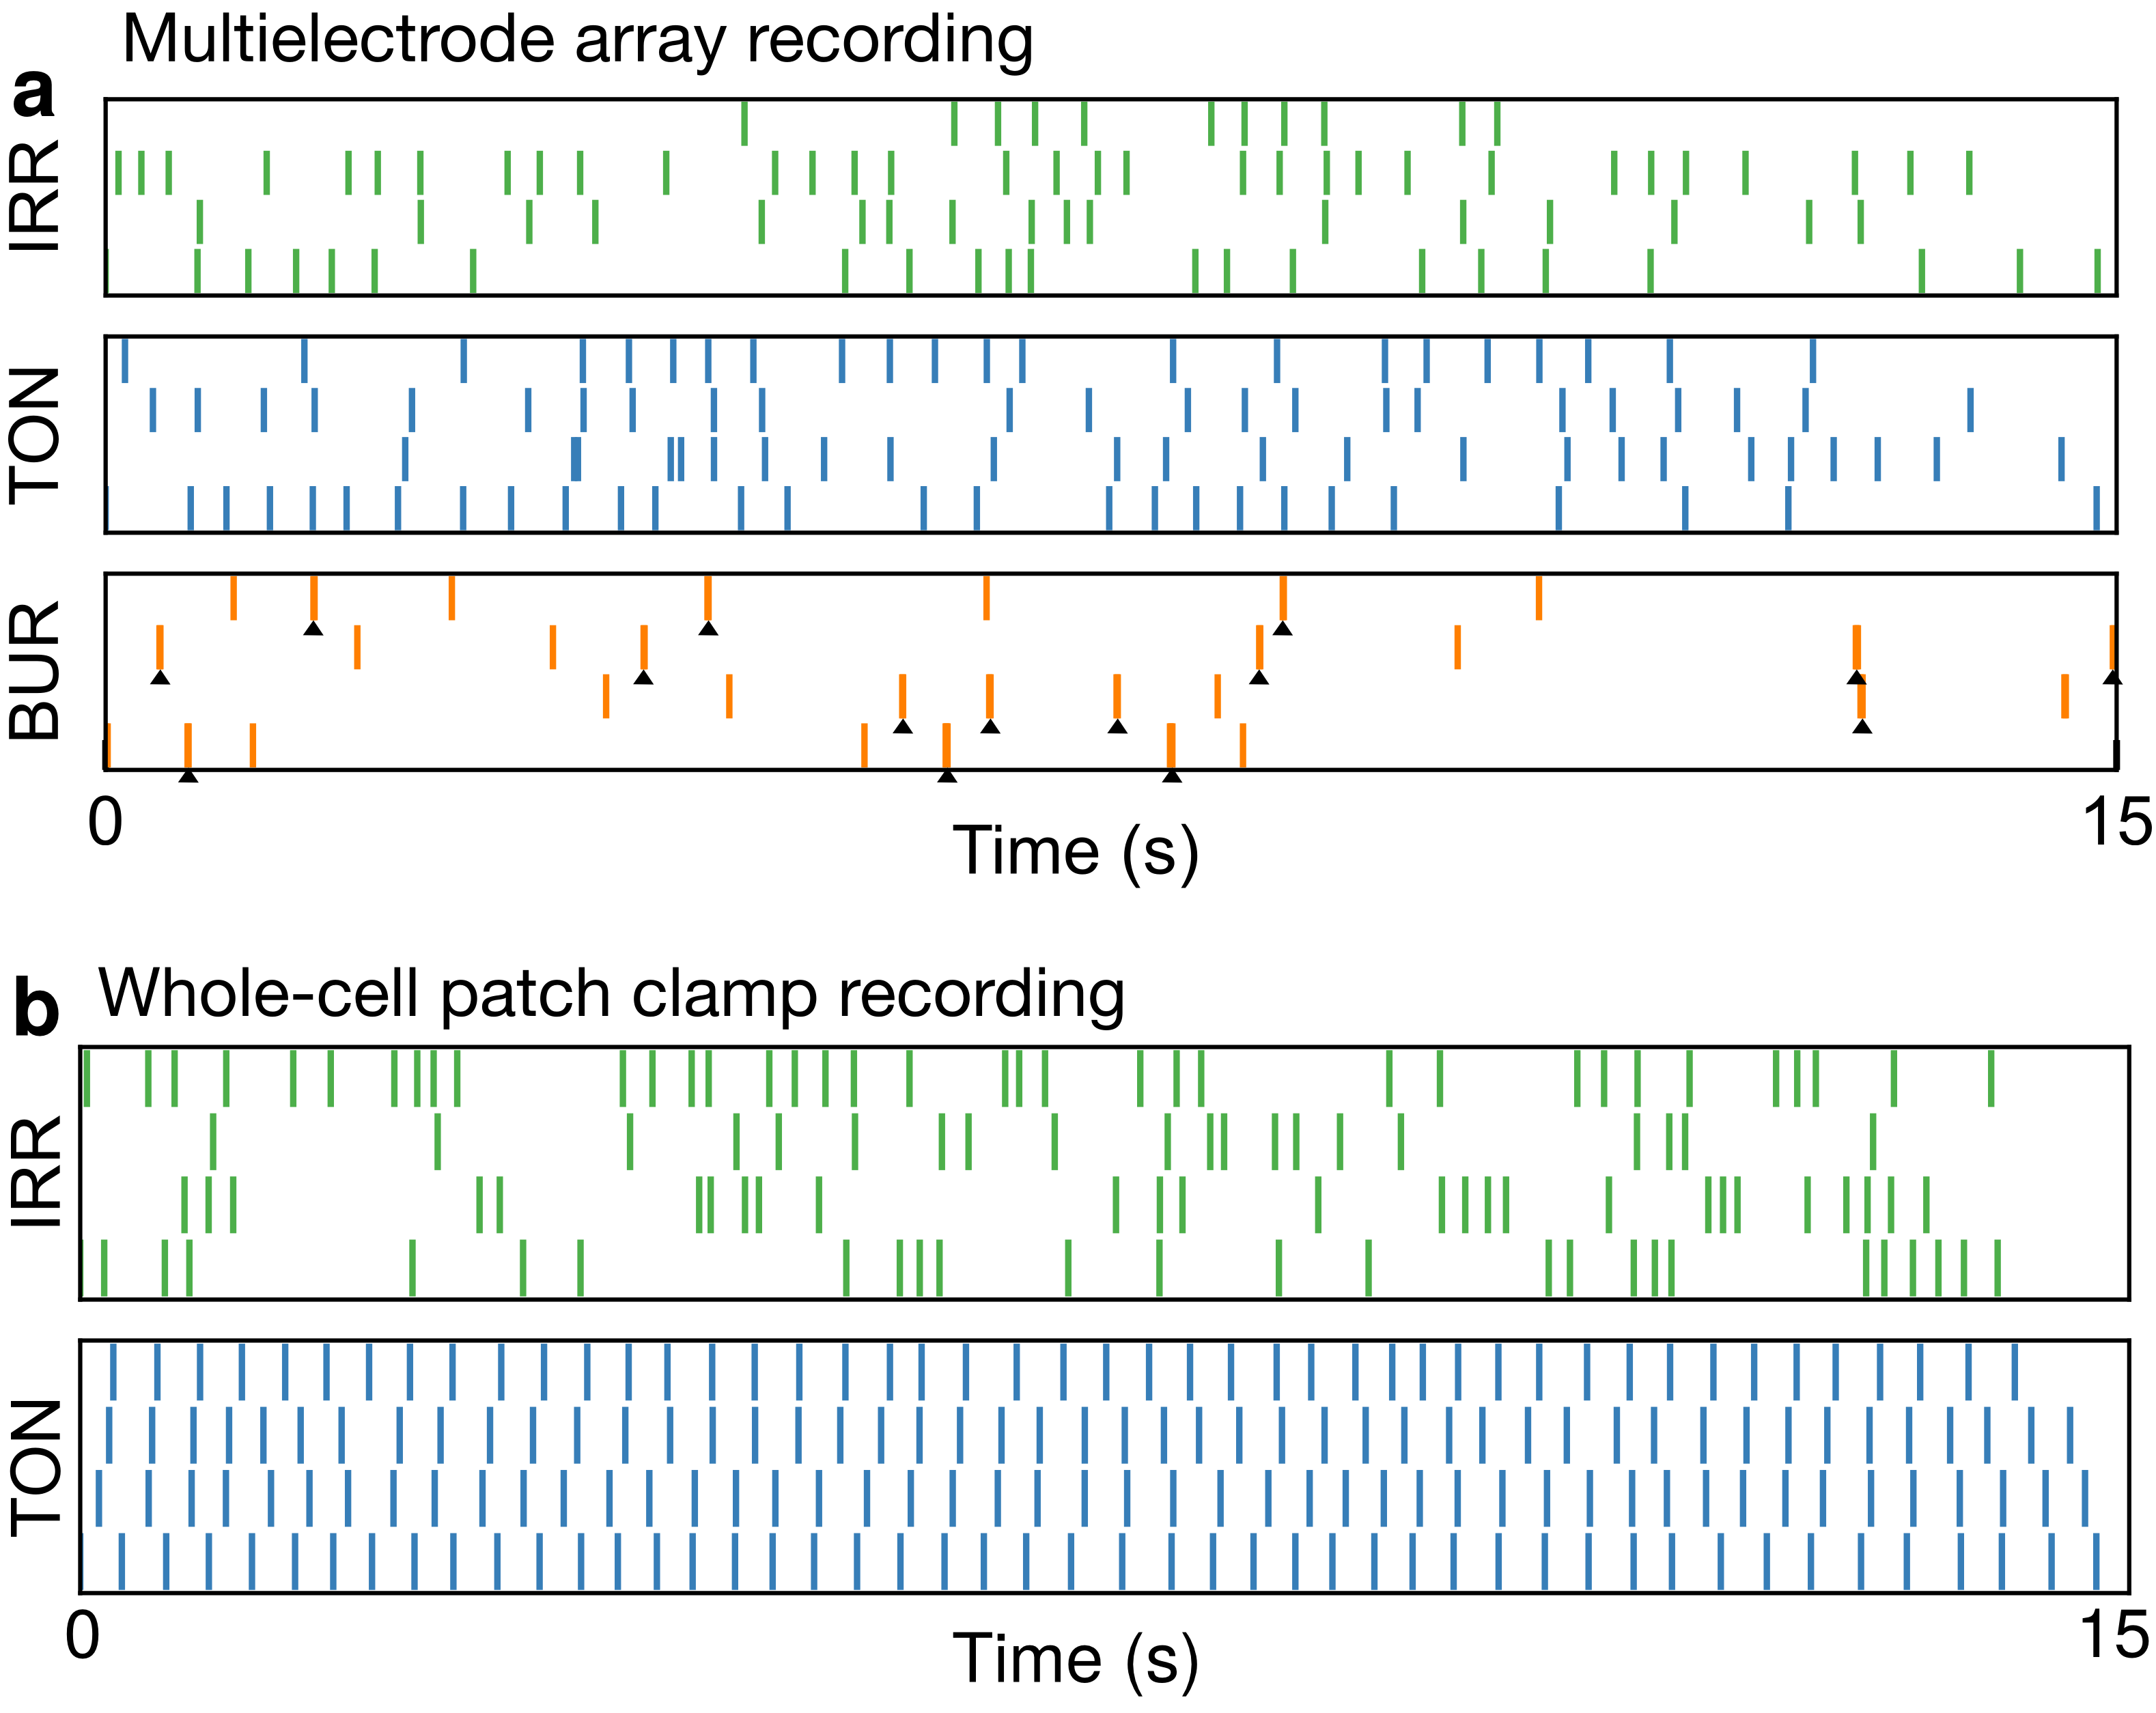
\includegraphics[width=3.5in]{chap5/figures/SupplementaryFigure4.png}
    \end{center}
    \caption{\label{fig:cms4} 
    Examples of SCN firing classes identified through hierarchical clustering
    (\textbf{a}) Representative examples of irregular, tonic and bursting firing in multielectrode array recordings. 
    (\textbf{b}) representative examples of irregular and tonic firing in whole-cell patch clamp recordings from Hermanstyne \textit{et al.} \cite{Hermanstyne2016}. 
    }
\end{figure}

\begin{figure}[p]
    \begin{center}
        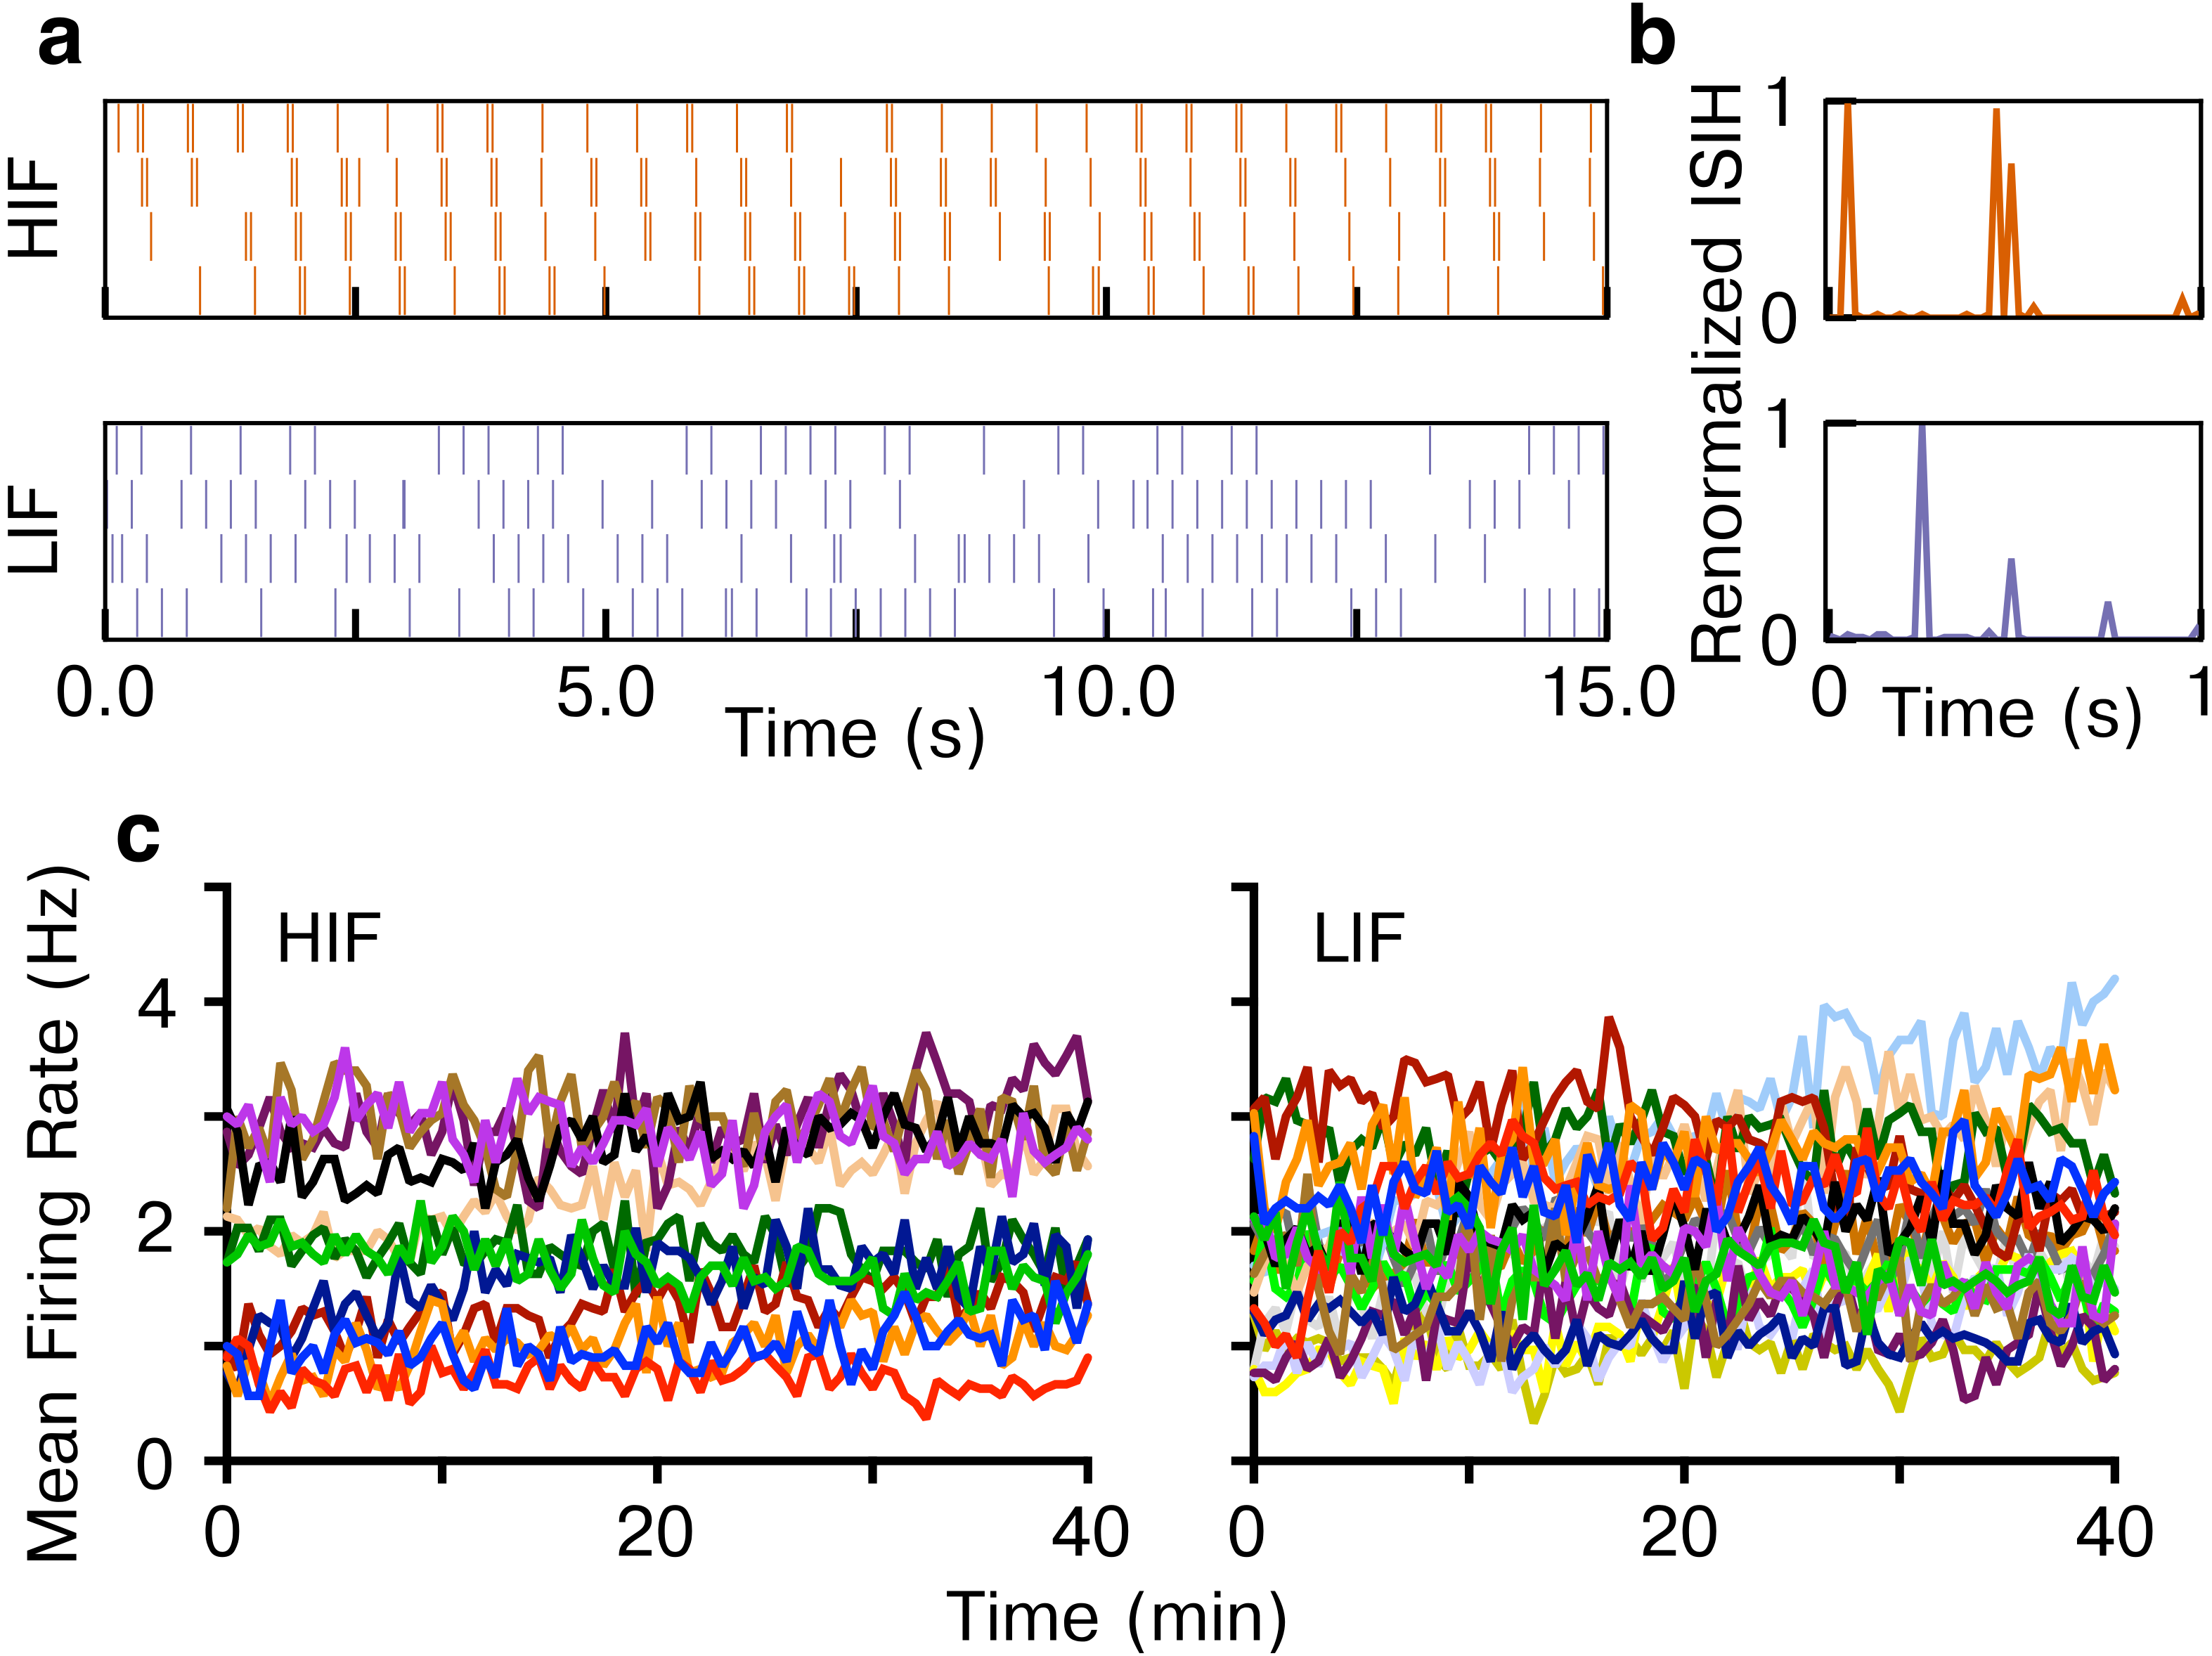
\includegraphics[width=3.5in]{chap5/figures/SupplementaryFigure5.png}
    \end{center}
    \caption{\label{fig:cms5} 
VIPChR2 neurons fire reliably in response to 40 min of HIF or LIF stimulation.
To test whether VIP neurons reliably fire at HIF and LIF frequencies, we stimulated VIPChR2 MEA cultures for 40 min with either frequency. 
(\textbf{a}) 60 s raster plots of two representative VIP neurons firing at HIF and LIF frequencies. The MEA recordings occasionally miss spikes (due largely to the proximity of a neuron to the electrode and the conservative clustering method) but the pattern of spike timing is consistent with the stimulation 
(\textbf{b}) as illustrated by the ISIH. 
(\textbf{c}) VIP firing binned at 30 s showed no change over a 40 min period with either HIF or LIF indicating that individual neurons show no evidence of habituation or depolarization block in response to HIF and LIF stimuluses. The neuron-to-neuron variability in mean frequency is likely primarily due to missing spikes on the multielectrode array.
    }
\end{figure}

\subsection*{High frequency stimulation of VIP neurons shifts genetic circadian rhythms \textit{in vitro}}


We next sought to test the role of the electrical activity we have identified within the SCN.
To do so, we optogenetically stimulated VIP neurons within SCN explant slice cultures and recorded circadian gene expression through the \textit{Per2}$^{Luc}$ bioluminescent reporter, which directly reports PER2 protein abundance).
We selected two firing patterns for the stimulation: low instantaneous frequency (LIF, 4 Hz), and high instantaneous frequency (HIF, 20 Hz doublets applied at 2 Hz).
These patterns share a mean firing rate across each second (4 Hz), but differ in spike timing.

Following several days of baseline recording, we stimulated VIP neurons with these patterns for 1 h near the peak of PER2 bioluminescence, corresponding to circadian time (CT) 9-12, since this time is associated with the largest response to exogenous VIP application \cite{An2011}
When applied to MEA SCN cultures, we found that 1 h stimulation did not result in depolarization block or habituation (Figure \ref{fig:cms5}).
We found that HIF stimulation resulted in phase delays of approximately 1.5 h, whereas LIF stimulation or stimulation of the control group did not (Figure \ref{fig:cm3}a-b). 
Furthermore, we found that stimulation in the presence of VIP antagonist significantly reduced the resulting phase shift (Figure \ref{fig:cm3}c).
Repeated stimulation for three days yielded similar results (Figure \ref{fig:cms6}.
Our results indicate that the phase of circadian gene expression is mediated through VIP release, which in turn is dependent upon firing frequency of VIP neurons.

\begin{figure}[p]
    \begin{center}
        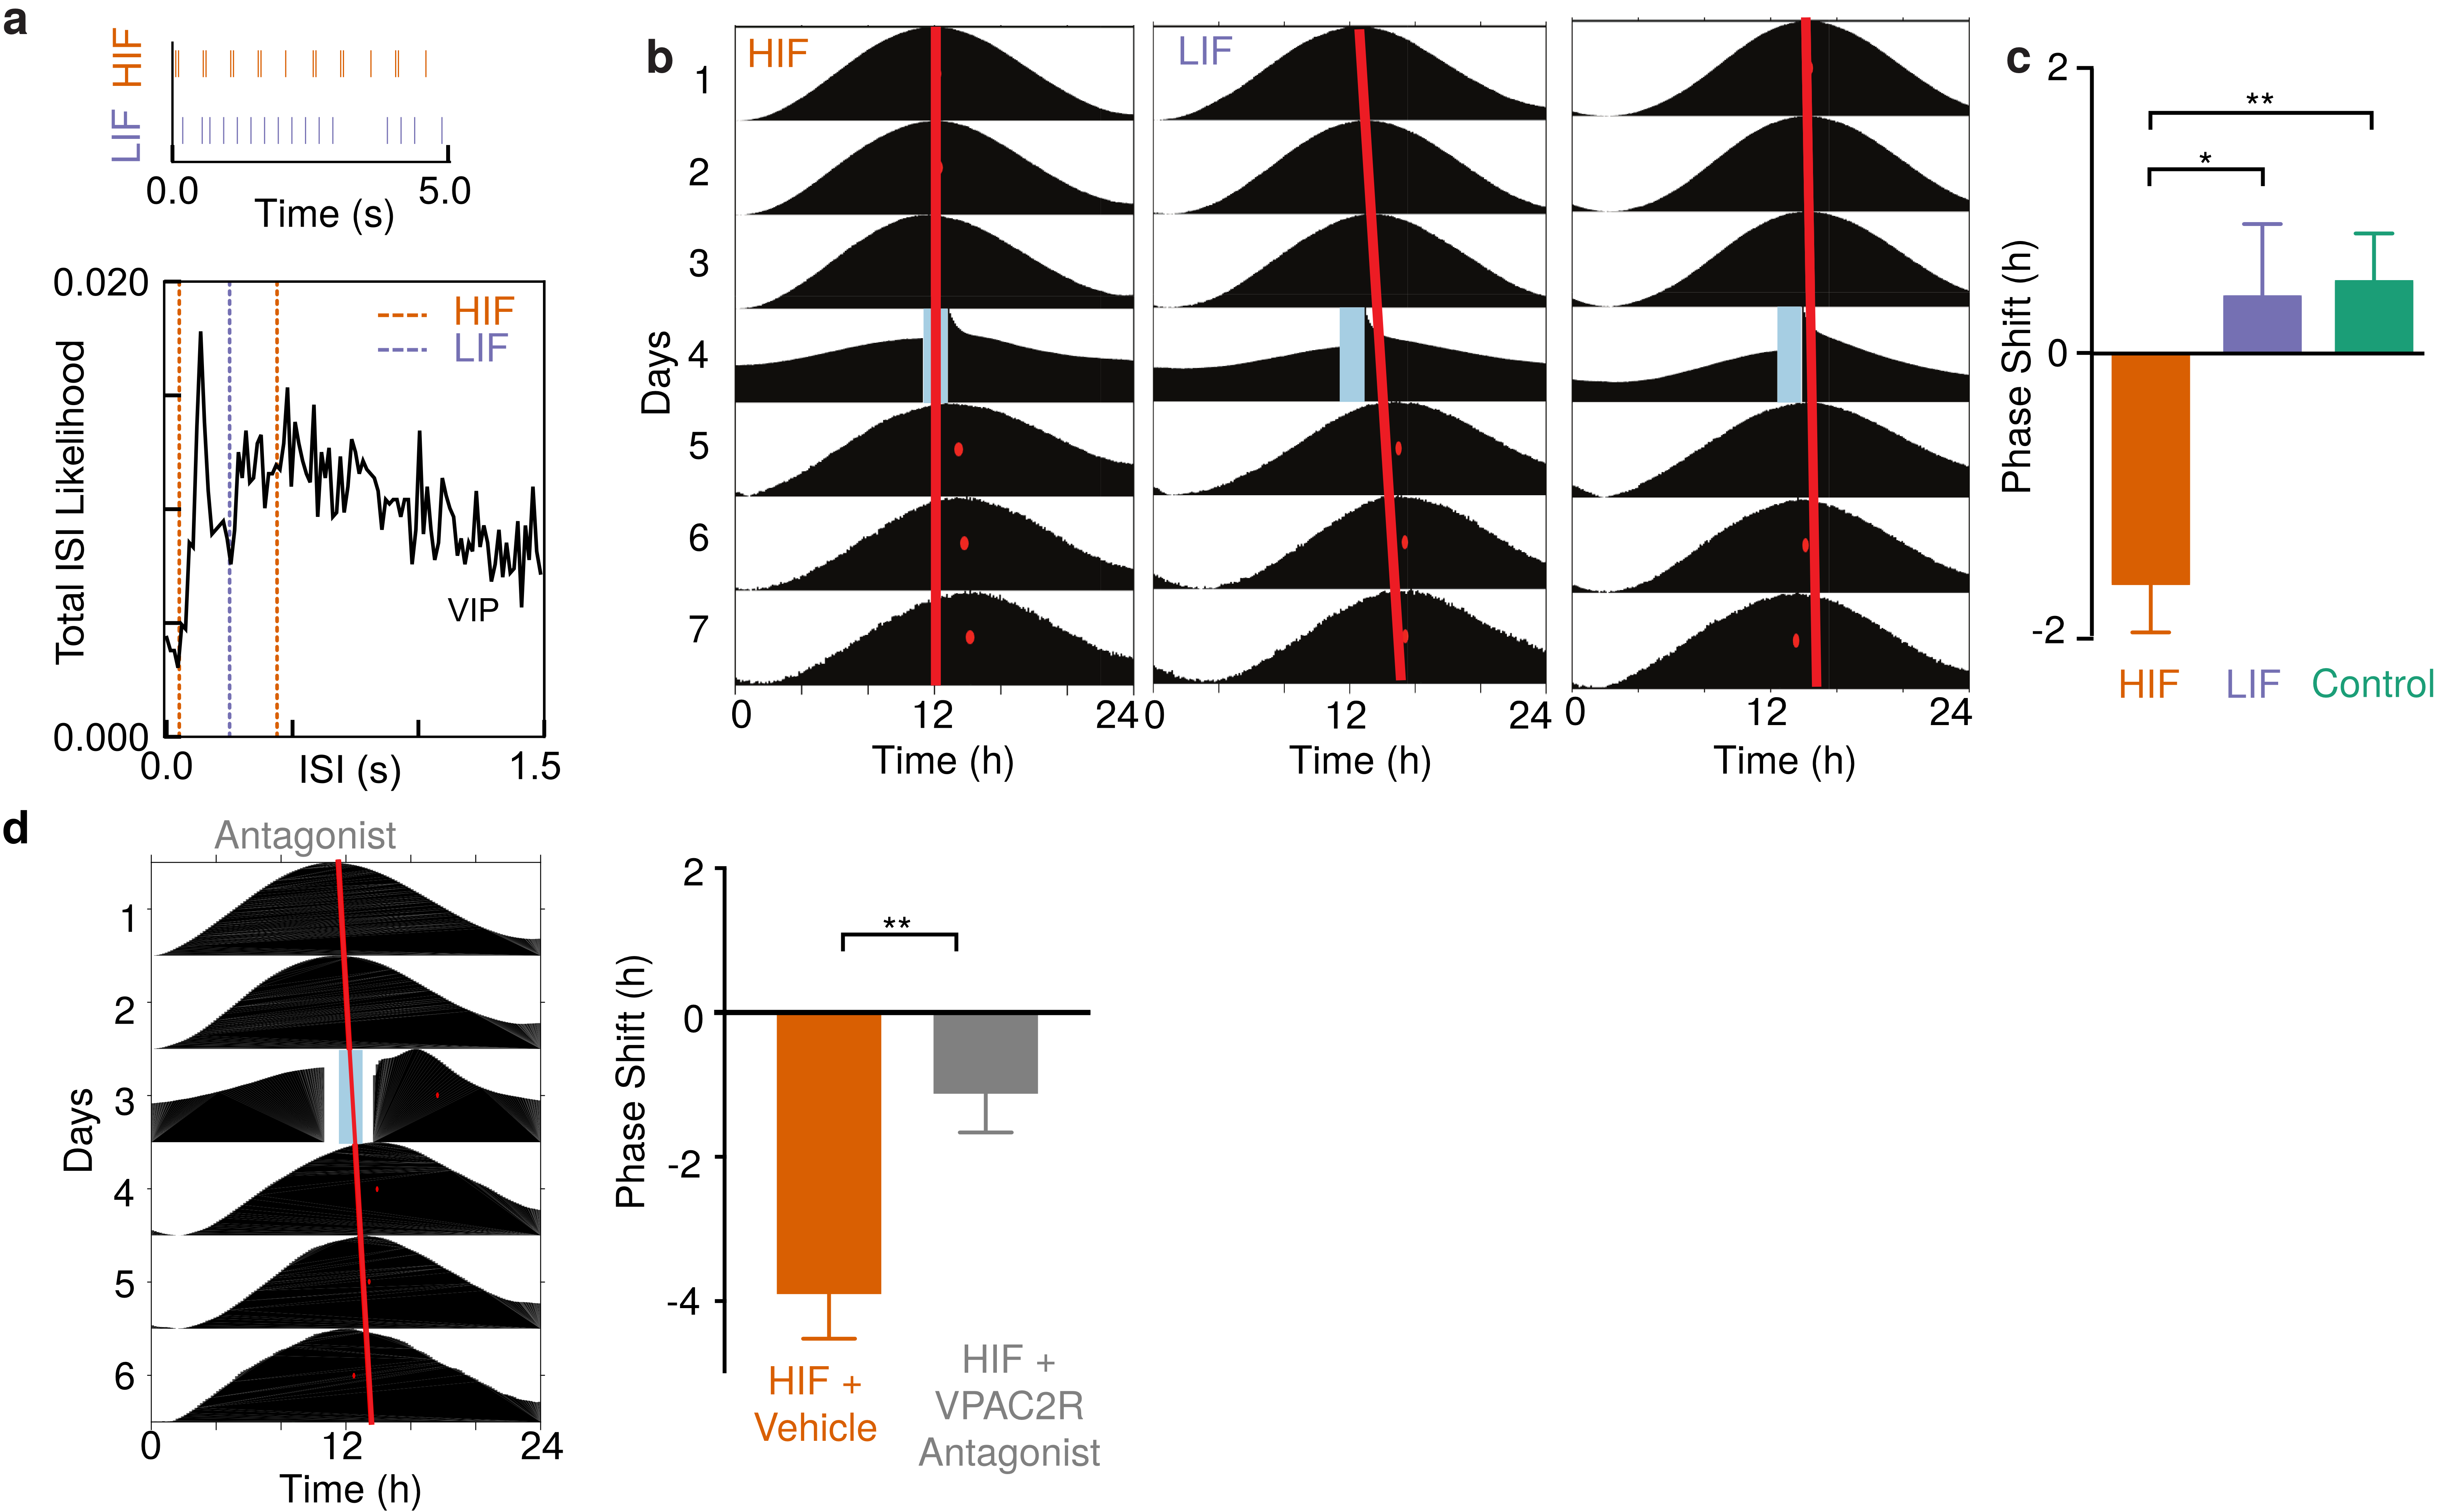
\includegraphics[width=6.5in]{chap5/figures/Figure3.png}
    \end{center}
    \caption{\label{fig:cm3} 
    High Frequency Optogenetic Stimulation of VIP SCN neurons phase delays circadian rhythms in PER2 expression. 
    (\textbf{a}) Optogenetic stimulation was selected from physiological relevant firing frequencies observed in VIP- specific multi-day multielectrode array recordings and whole-cell slice recordings. High instantaneous frequency stimulation (HIF) and low instantaneous frequency stimulation (LIF) evoke similar numbers of action potentials with dramatically different interspike intervals. 
    (\textbf{b}) Representative \textit{Per2}$^{Luc}$ actograms from three SCN slices. In the top two traces, ChR2 expressed in VIP neurons was activated for 1 h (blue bar) on the fourth day of recording with high (HIF) or low (LIF) frequencies. Control SCN received either HIF or LIF stimulation, but lacked ChR2. Note the large delay in the time of the daily PER2 (red dots) on the days after HIF stimulation relative to the extrapolated unperturbed phase (red line). 
    (\textbf{c}) HIF stably delayed PER2 rhythms compared to either LIF or control conditions ($-1.6 \pm 0.3$ h, HIF, $0.4 \pm 0.5$, LIF, $0.5 \pm 0.3$, control; *$P < 0.05$ and **$P < 0.01$, one-way ANOVA with Tukey’s posthoc test, n= 9, 10 and 32 SCN slices, respectively). 
    (\textbf{d}) VPAC2 antagonist treatment during HIF stimulation reliably reduces the resulting phase shift, shown by a representative actogram (left) and the group summary. ($-3.902 \pm 0.6178$ HIF + Vehicle, $-1.124 \pm 0.5381$ HIF + VPAC2R Antagonist; **$P < 0.01$, unpaired t-test, $n =  7,7$ SCN slices, respectively). 
    }
\end{figure}

\begin{figure}[p]
    \begin{center}
        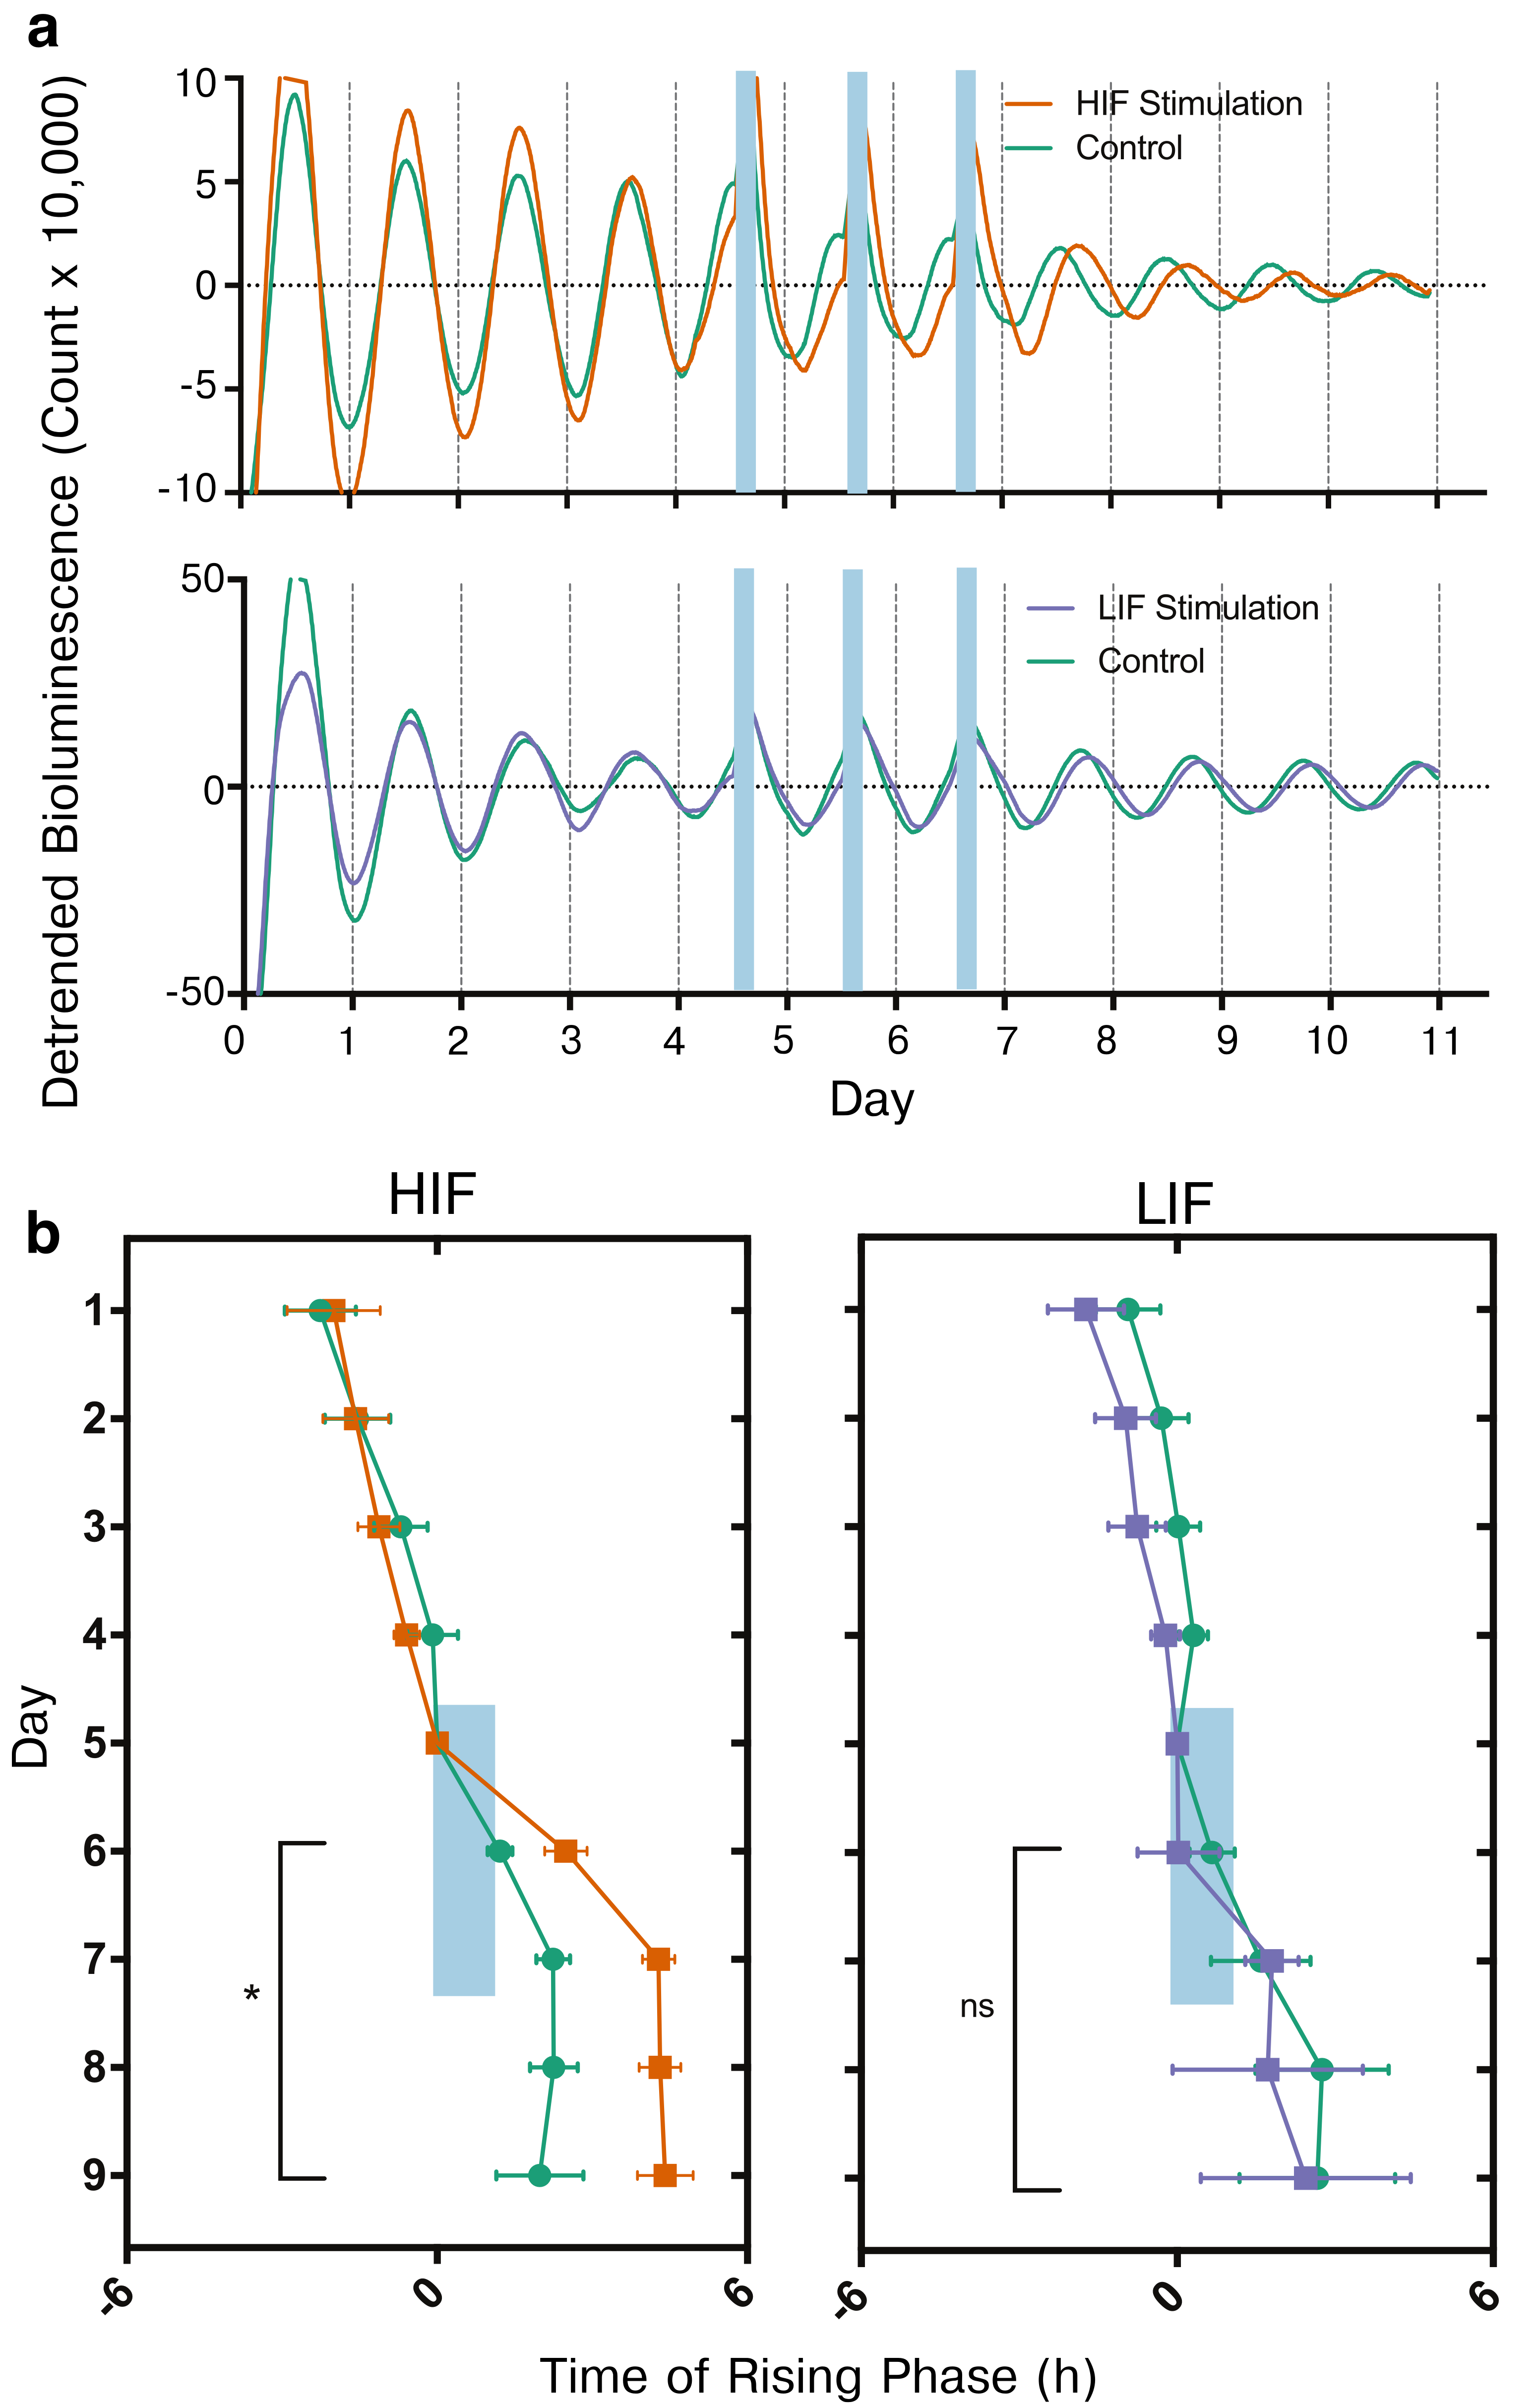
\includegraphics[width=3.5in]{chap5/figures/SupplementaryFigure6.png}
    \end{center}
    \caption{\label{fig:cms6} HIF but not LIF stimulation of VIP neurons shifts clock gene rhythms in SCN slices. 
    (\textbf{a}) Representative bioluminescence traces show that daily HIF stimulation (blue bars) phase delayed PER2 circadian rhythms compared to control SCN explants, while LIF stimulation did not. 
    (\textbf{b}) Using the rising phase as a reliable phase marker, we found that HIF stimulation sufficed to change the phase of PER2 expression compared to controls ($n = 8$ VIPChR2, and $n=7$ control, Watson-Williams test for days 6 – 9, *$P< 0.05$). LIF stimulation failed to phase shift PER2 gene expression ($n = 5$ VIPChR2 SCN, and $n = 10$ control SCN, Watson-Williams test for days 6-9, $P = 0.5$).
    }
\end{figure}

\subsection*{High frequency stimulation of VIP neurons induces cFOS expression throughout the entire SCN \textit{in vivo}}
Next, we sought to determine if VIP neuronal stimulation resulted in neurotransmission throughout the SCN.
VIP neurons are predominantly located in the ventrolateral SCN, though they densely innervate the rest of the SCN, and the VPAC2R VIP receptor is expressed throughout the SCN \cite{An2012}.
Consistent with our expectation, we found that \textit{in vivo} stimulation of VIP neurons increases expression of cFOS, a marker of neuronal activation, throughout the SCN (Figure \ref{fig:cm4}).
Expression of cFOS increased approximately 5-fold in the ventral SCN, and 4-fold in the dorsal SCN compared to controls.
Thus, \textit{in vivo} stimulation of VIP neurons increases the electrical activity in both VIP and nonVIP subpopulations of the SCN.
\clearpage
\begin{figure}[p]
    \begin{center}
        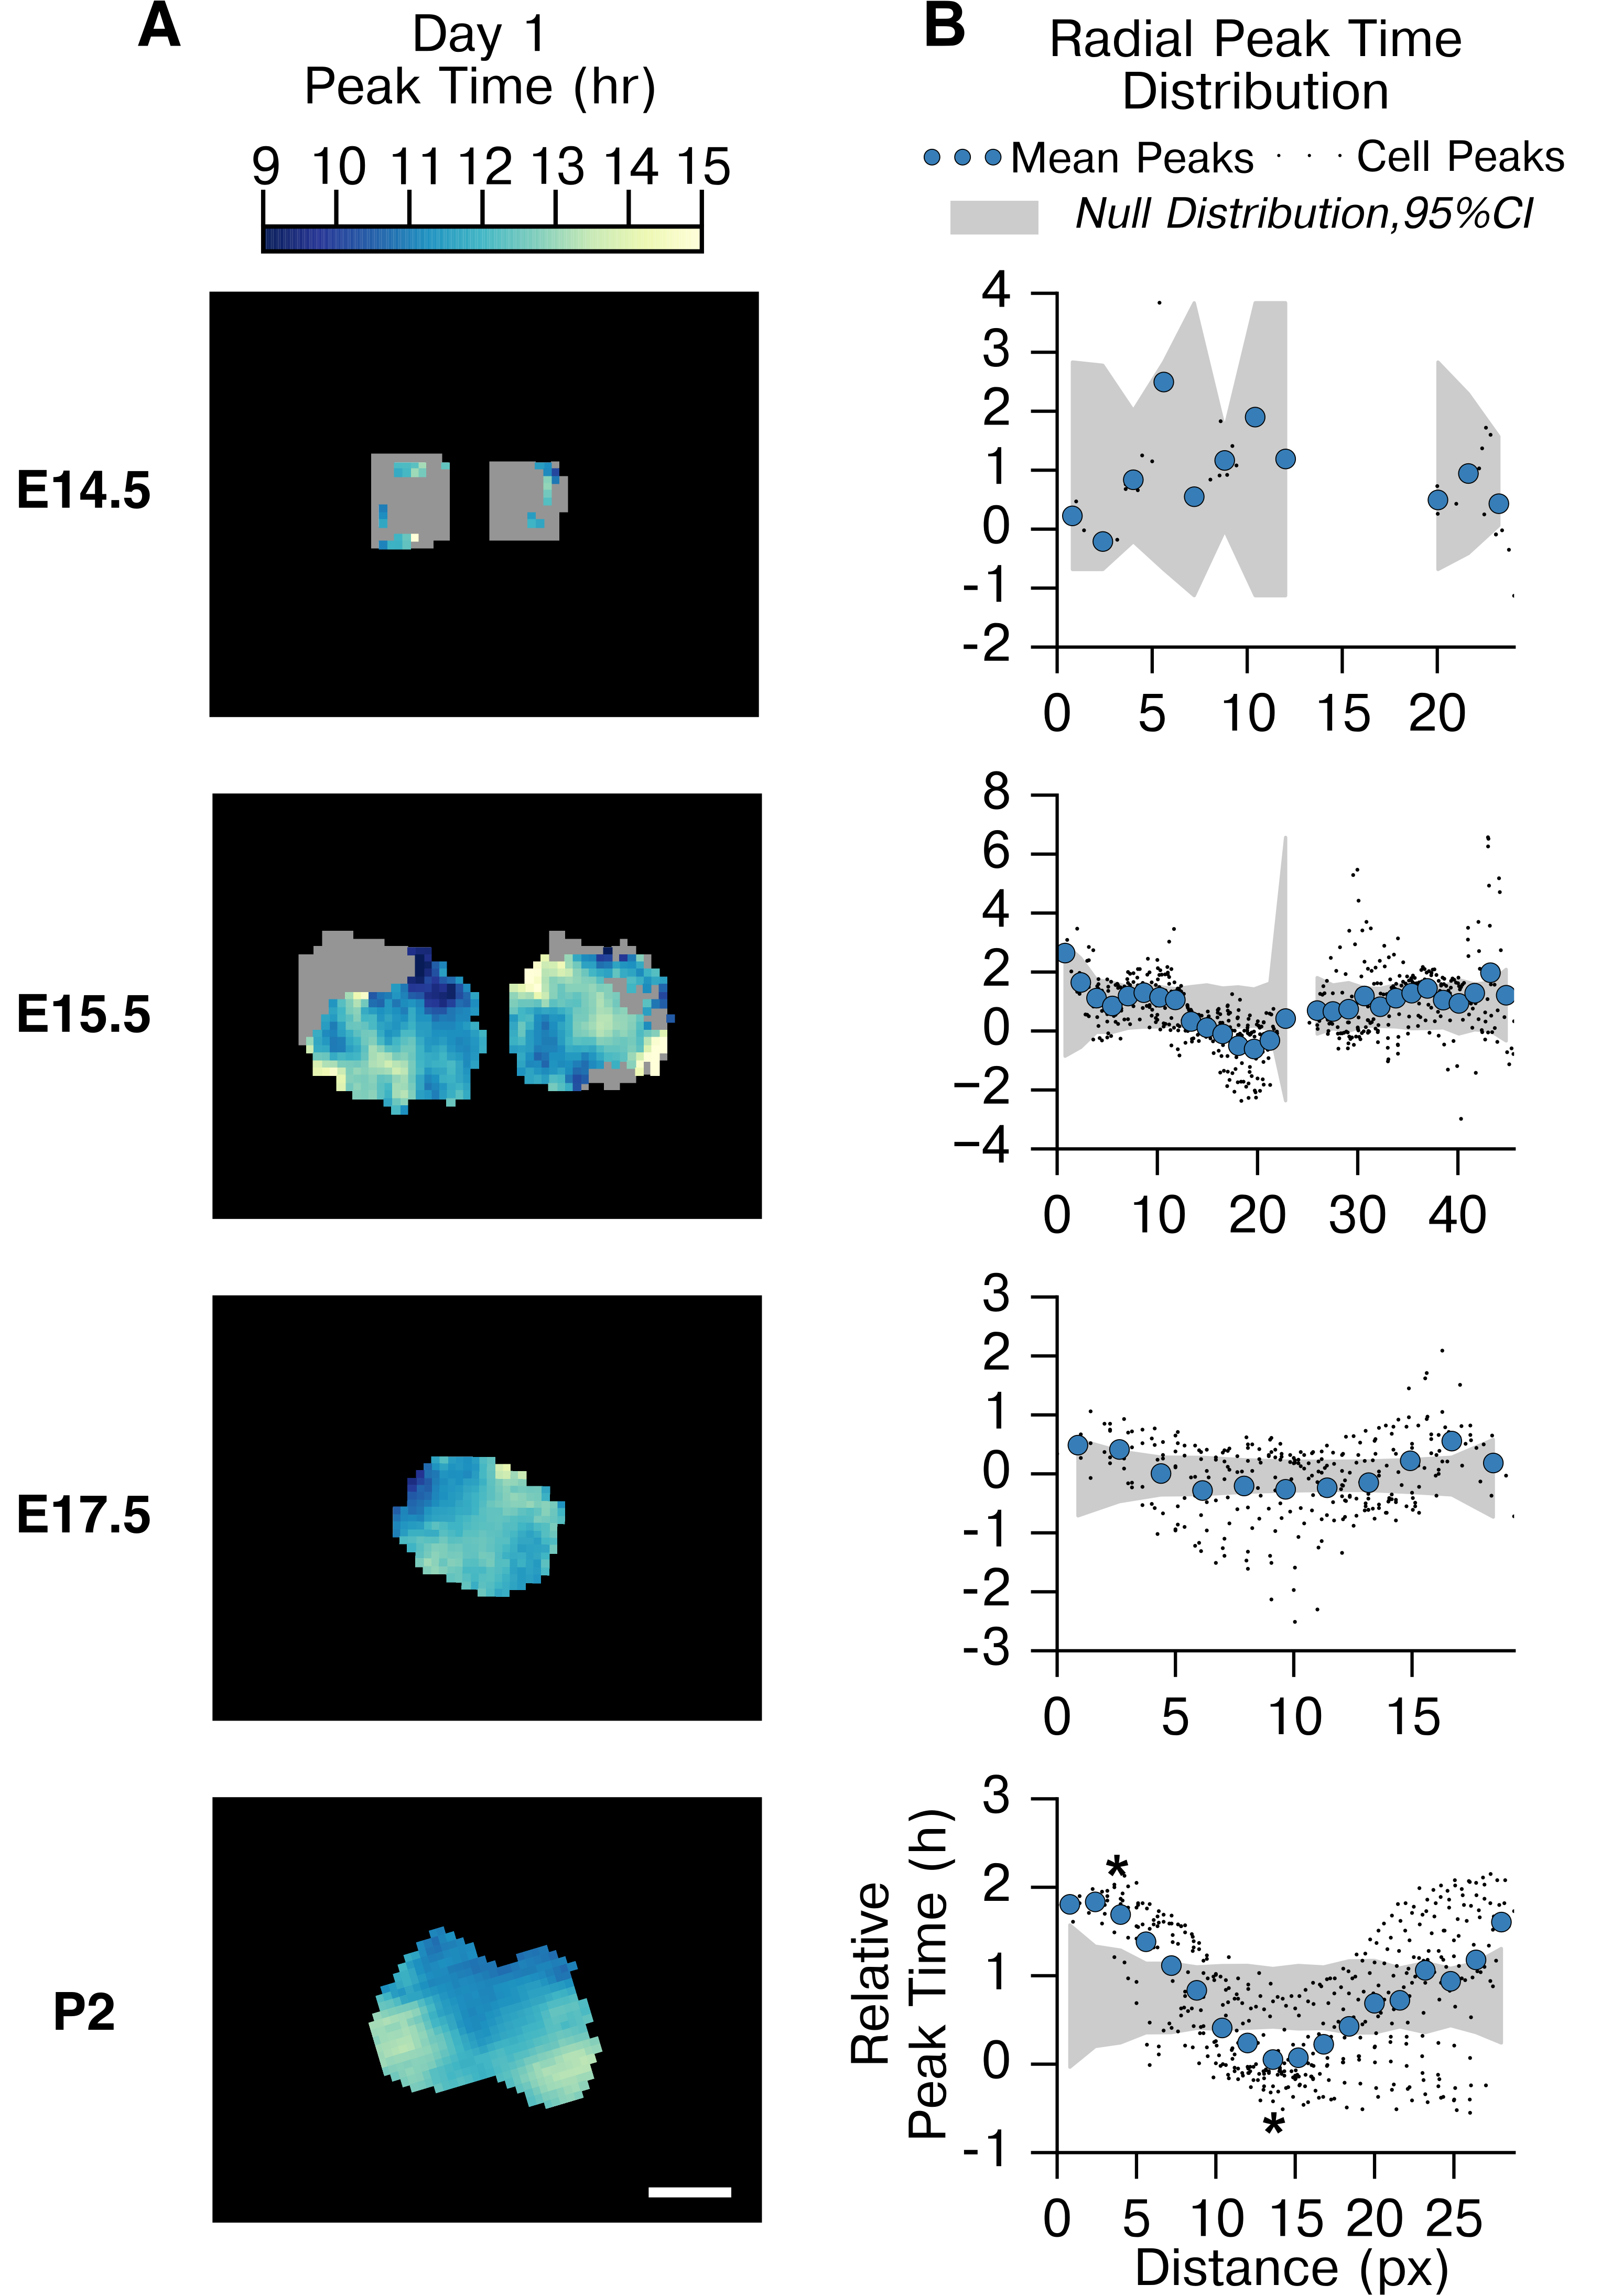
\includegraphics[width=3.5in]{chap5/figures/Figure4.png}
    \end{center}
    \caption{\label{fig:cm4} Activation of SCN VIP neurons in vivo induces cFOS expression throughout the SCN. 
    (\textbf{a}) Representative image of the bilateral SCN showing cFOS induction (magenta) within VIPChR2 neurons (yellow) after 1 h of 15 Hz stimulation in vivo at CT13 (scale bar = 100 $\mu$m). 
    (\textbf{b}) The number of SCN cells expressing cFOS protein was higher in VIPChR2 (bottom) than control (top panel) mice after 1 h of 15 Hz stimulation at CT13. \textit{In vivo} optogenetic stimulation of VIP neurons increased cFOS expression throughout the SCN (577.8 ± 33.0 Ventral SCN VIPChR2, $103.0 \pm 56.9$ Ventral SCN Control, $244.5 \pm 15.6$ Dorsal SCN VIPChR2, $63.0 \pm 17.9$ Dorsal SCN Control; unpaired Student's t-test ***$P<0.001$, $n = 4$ mice for each condition).
    }
\end{figure}

\clearpage
\subsection*{High and low frequency stimulation of VIP neurons entrains daily locomotor rhythms \textit{in vivo}}

Next, we used daily wheel running activity as a marker for circadian phase to investigate the role of VIP neuronal firing and frequency on behavioral circadian rhythms \textit{in vivo}.
Control and VIPChR2 mice were enucleated to prevent response to ambient light input, and a fiber optic cannula was implanted to deliver light for optogenetic stimulation of VIP neurons in the SCN.
Enucleated mice, as in darkness, display a free-running circadian rhythm with a near-24 h periodicity (period $=23.4\pm0.1$, $n=7$ VIPChR2, period $=23.4\pm0.2$, $n=4$ control).

To first test if stimulation of VIP neurons alone was sufficient for entrainment, two VIPChR2 and one control mice were delivered 1 h of optogenetic stimulation each day for up to 30 days with a HIF pattern (Figure \ref{fig:cm5}a), resulting in entrainment only in the case of the VIPChR2 mice.
Next, HIF and LIF stimulation was applied for 1 h each day for a minimum of four days in a randomized order (HIF then LIF, or LIF then HIF), with four days of no stimulation and free-running circadian behavior between HIF/LIF patterns.
From these data, we calculated a phase response curve for the 1 h stimulus (combined HIF and LIF, Figure \ref{fig:cm5}b).
Control mice showed no response, whereas VIPChR2 mice displayed solely phase delays primarily in the early to mid subjective night (CT10-18), which were sufficient for entrainment.
Interestingly, optogenetic stimulation in VIPChR2, but not control, mice resulted in an acute reduction in wheel running activity during the early subjective night (CT12-18, mouse activity primarily occurs during these times and so stimulation effects of acute activity at CT0-12 and CT18-24 could not be tested).
Light evokes similar suppression of mouse activity in subjective night, though the mechanism by which this occurs is unknown.

Finally, we compared the ability of HIF and LIF to entrain mouse behavior (Figure \ref{fig:cm6}).
We found that although both HIF and LIF were able to entrain locomotor activity, mice under HIF condition entrained more rapidly.
In conjunction with our \textit{in vitro} assessment of circadian phase shifting, we conclude therefore that firing frequency affects the magnitude of phase shifting possibly through altering the likelihood of VIP release.
\clearpage
\begin{figure}[p]
    \begin{center}
        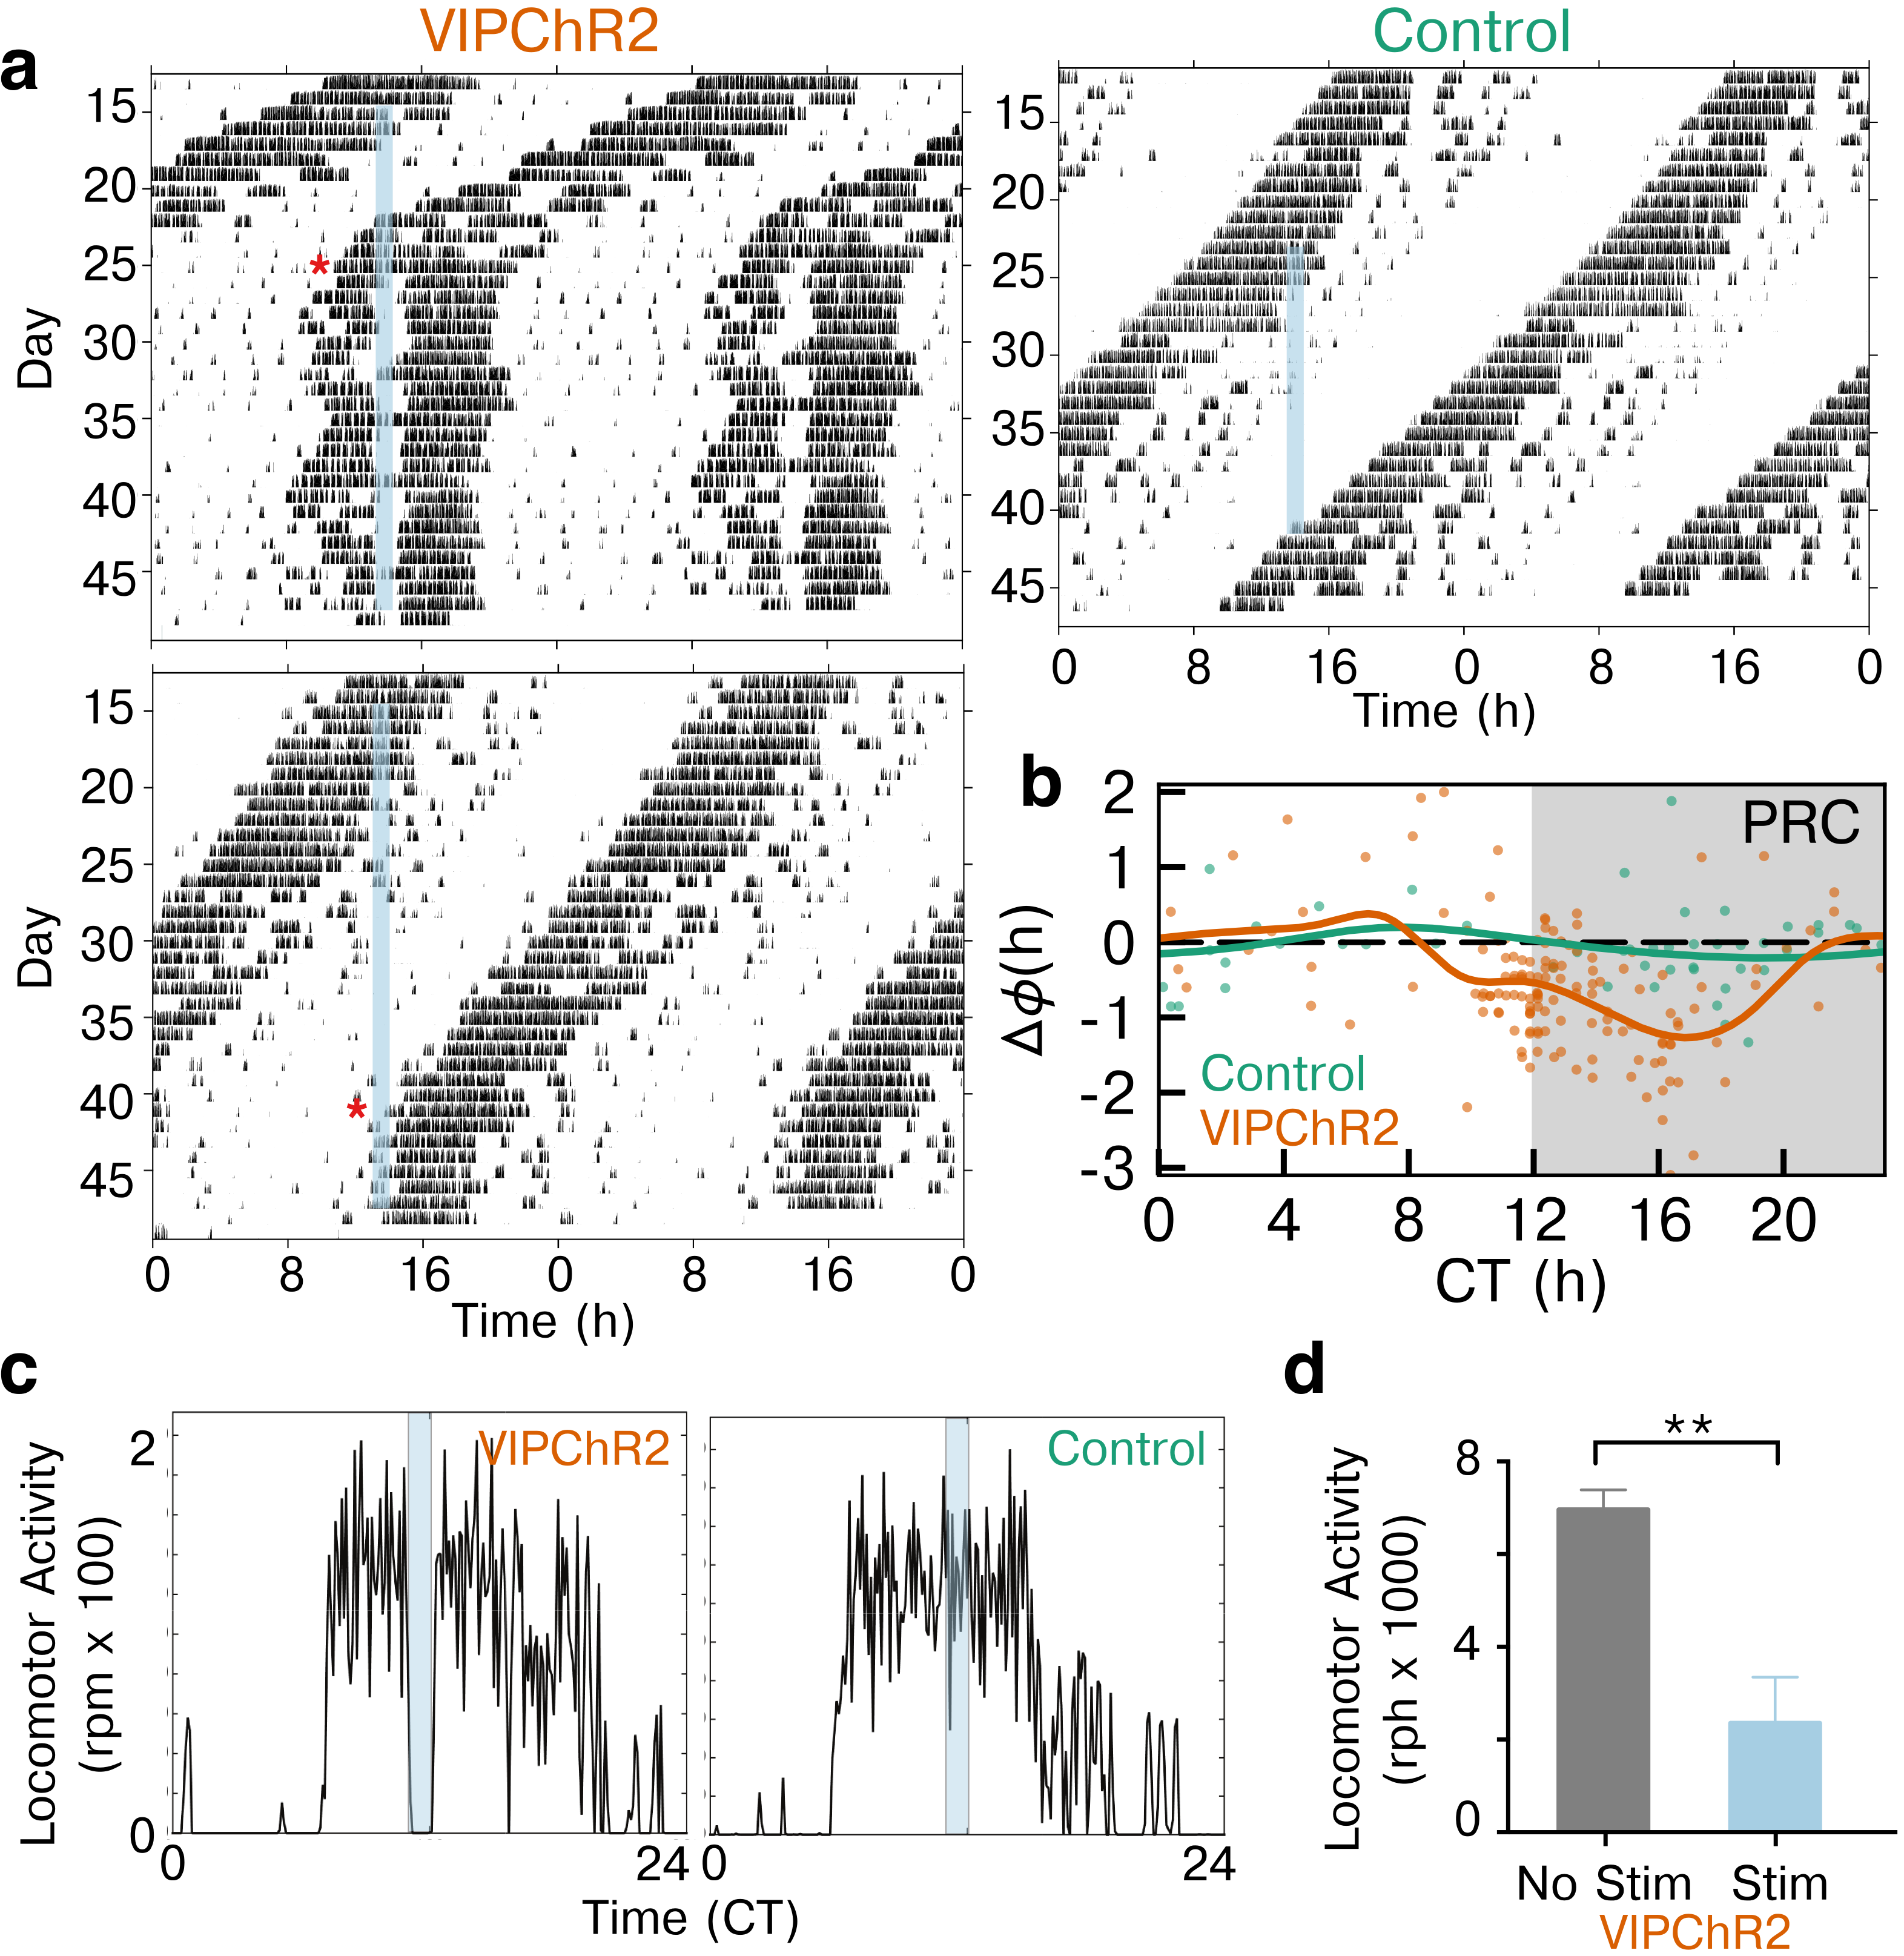
\includegraphics[width=4.5in]{chap5/figures/Figure5.png}
    \end{center}
    \caption{\label{fig:cm5}
    Optogenetic stimulation of only VIP neurons \textit{in vivo} entrains locomotor activity. 
    (\textbf{a}) Daily locomotor activity of two representative mice entrained to HIF stimulation of SCN VIP neurons (blue bar) compared to a control mouse lacking ChR2. Actograms show wheel revolutions per 6 min (black bars) recorded from enucleated mice for almost 50 days. Note that the two VIPChR2 mice, with slightly different periods, reached stable entrainment (*) only when the stimulation occurred around early subjective night. 
    (\textbf{b}) Average phase response curves for HIF and LIF stimulation of VIPChR2 (orange, $n = 7$) and control mice (green, $n = 4$) show the change in phase (dots) on the day after stimulation at different circadian times. Note that activation of VIP neurons entrained daily locomotor rhythms through phase delays when delivered during the late subjective day and early subjective night.
    (\textbf{c}) Representative activity profiles of 2 mice show that HIF stimulation of VIP neurons acutely reduced running wheel activity in VIPChR2 (left), but not control (right), mice. 
    (\textbf{d}) Wheel revolutions during optogenetic stimulation (CT 12-18, 1 h of HIF) decreased nearly four-fold compared to baseline in VIPChR2 mice ($2355.0 \pm 981.1$ during stimulation vs. $6958.0 \pm 418.9$ with no stimulation, $n = 6$ mice, paired Student's t-test **$P< 0.01$). 
    }
\end{figure}
\clearpage
\begin{figure}[p]
    \begin{center}
        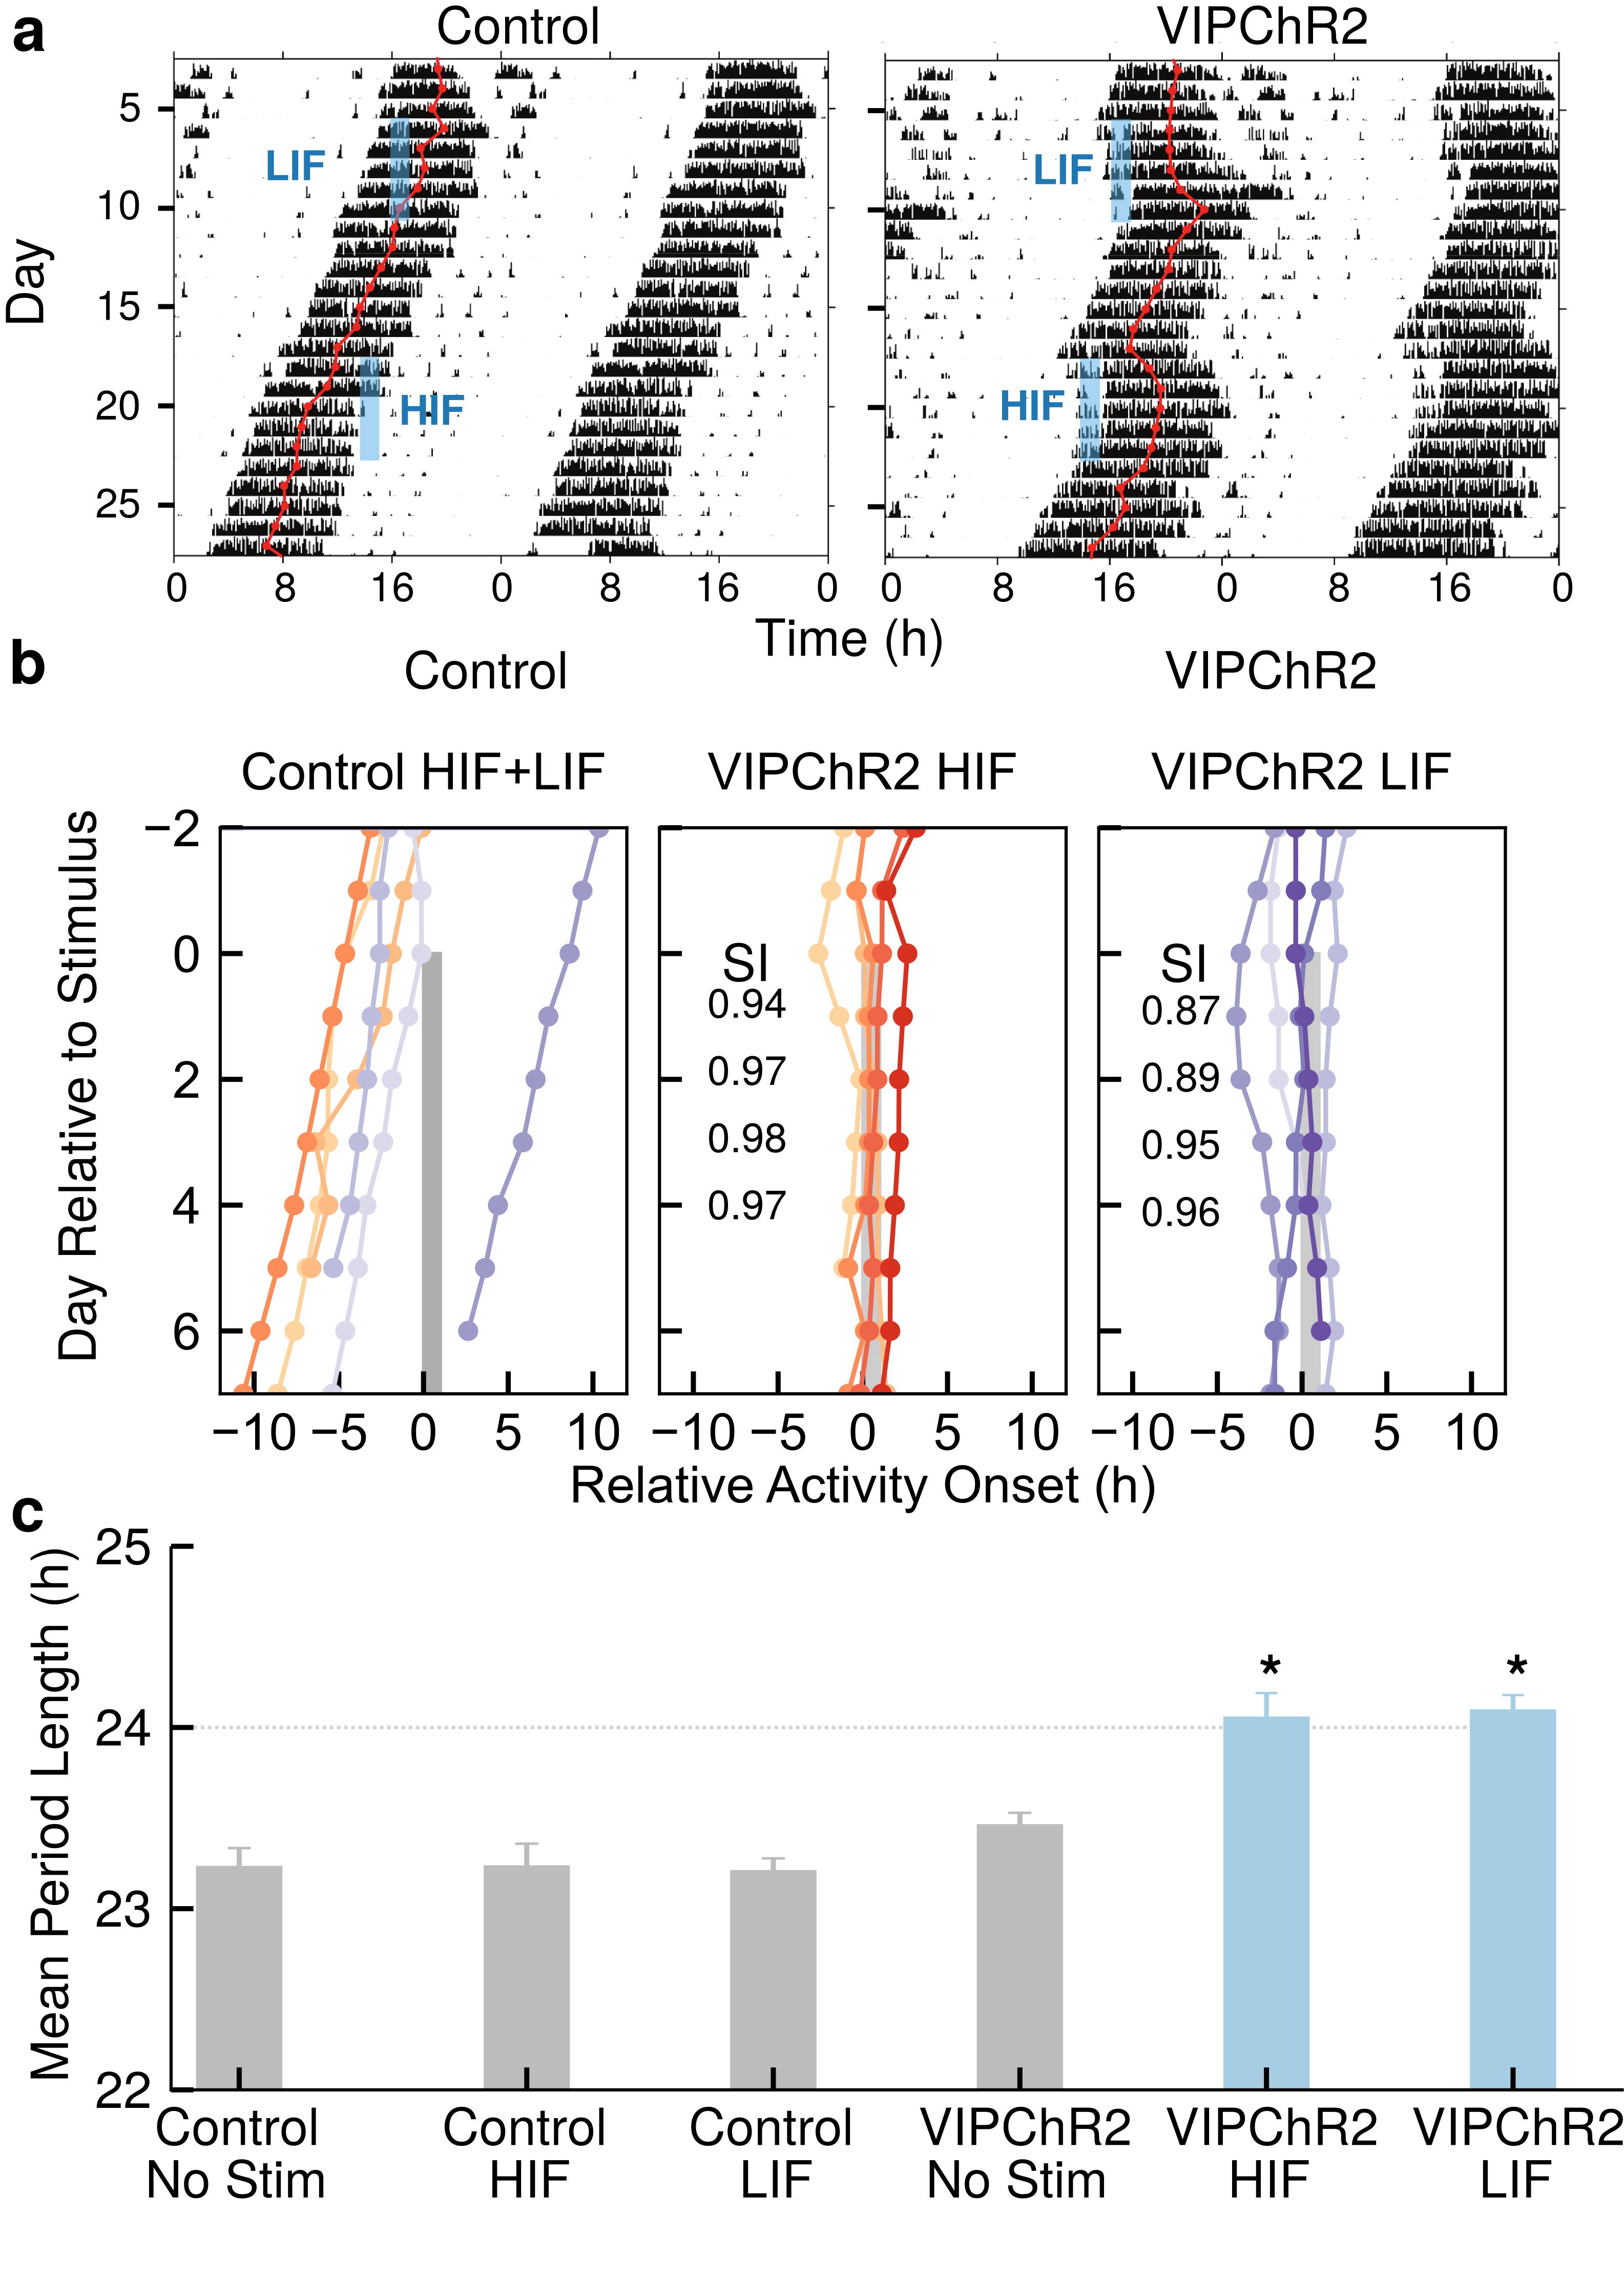
\includegraphics[width=3.5in]{chap5/figures/Figure6.png}
    \end{center}
    \caption{\label{fig:cm6} Instantaneous firing pattern affects locomotor rhythm entrainment.
    (\textbf{a}) Representative actograms show how daily optogenetic stimulation with HIF or LIF (blue bar) differentially entrained VIPChR2, but not control, mice. The daily acrophase (red circles and lines) of control mice in constant darkness free-ran through the days of stimulation. In contrast, daily HIF stimulation produced a large delay and rapidly entrained locomotor rhythms. Daily LIF stimulation, though having smaller effects on phase, also entrained activity.
    (\textbf{b}) Daily stimulation entrained daily activity onsets to within 2 h of the stimulation in both HIF and LIF but not in control mice. HIF stimulation immediately resulted in tight clustering fo activity onsets, as shown by the higher synchrony index (SI), while LIF stimulation more gradually entrained to the stimulation, as seen by the gradually increasing SI. 
    (\textbf{c}) Daily HIF or LIF stimulation shifted the period of locomotor rhythms to 24 h in VIPChR2, but not control, mice (one-way ANOVA with posthoc Tukey HSD *$P < 0.05$). Note that VIPChR2 mice displayed a period identical to controls while stimulation was off, indicating that it was activation of VIP neurons causing a 24 h period rather than simply the genotype.
    }
\end{figure}



\clearpage
\section{Discussion}
In this chapter we sought to relate electrophysiological properties of a distinct subset of SCN neurons with their previously-known neurotransmitter content and role in SCN synchrony and entrainment.
Most intriguingly, we found that there are further subclasses of neurons within the subset of SCN neurons that express VIP, as identified by spontaneous firing patterns.
The persistent and heterogeneous firing patterns within this subpopulation suggests multiple specific roles for these firing patterns in SCN function.
Other studies have presented some evidence for multiple subpopulations of VIP-expressing SCN neurons that arise at different times in development \cite{Ban1997}, however it is unknown if these developmental subpopulations correspond to the electrophysiological subpopulations we have identified.
It is possible that these patterns are reflective of differing connectivity, such as receiving retinal input or projecting within or outside of the SCN to establish synchrony or entrainment.
Further study is needed to characterize the projections from VIP SCN neurons, and determine how this might be correlated with firing pattern and thus neuropeptide release.

The phase responses we observed following stimulation of VIP neurons only partially recaptures the phase responses observed during whole-SCN optogenetic stimulation \cite{Jones2015}.
This is unsurprising, as there are numerous pathways of neurotransmission in the SCN, and the phase response curves calculated by Jones \textit{et al.} are likely the dynamic response to the simultaneous activation of many pathways.
Because approximately half of nonVIP neurons we tracked were found to also have circadian rhythms in electrical activity, it remains an open question as to which neurotransmitters are released at which phases in the course of a normal day of circadian oscillation \textit{in vivo}, and what their effects might be.
Based on our observation that VIP stimulation evoked only phase delays, we speculate that each subpopulation of SCN neurons may play differing roles in maintaining the stability of phase relationships and entrainment in the SCN.
Further evidence for this idea has recently been presented by studies of AVP-expressing neurons of the SCN \cite{Mieda2015}.
Though the numerous pathways present in the SCN at first may seem divergent in roles and thus imposing to characterize, there is some hope that they ultimately may be understood by their effect on phosphorylational states of clock products and clock inputs such as CREB \cite{Herzog2017, Aton2006, Bedont2015, Bieler2014, Liu2007a, Maywood2007}.

Interestingly, stimulation of VIP neurons also resulted in acute cessation of locomotor activity.
This is consistent with a previous study showing that SCN electrical activity was correlated with locomotor inactivity \cite{Vanoosterhout2012}.
There, the authors suggested that it was activity that suppressed SCN firing and thus activity could be considered an input into the clock.
Here, we found a causal relationship in the opposite direction: stimulation of the SCN resulted in suppression of activity, rather than activity resulting in the suppression of SCN firing.
Furthermore, how VIP neurons connect to behavioral circuits remains unknown.

We also found that the instantaneous firing frequency affects the phase shifts caused by VIP neurons.
Importantly, quantification of the actual release of VIP within the SCN in response to stimulation at different frequencies remains a significant experimental challenge.
Prior studies studies have shown that neuropeptide release can be caused by increases in either cytosolic  Ca$^{2+}$ as well as local Ca$^{2+}$ influx in microdomains of the synaptic terminal \cite{Verhage1991}.
Thus, it is possible that instantaneous frequency affects the total local or cytosolic Ca$^{2+}$ concentration, and thus the amount of VIP released.
A potential approach to address this question is through the use of a VIP-sensing fluorescent reporter (VIP-SnFR) as has been done previously for glutamate \cite{Marvin2013}.
Another potential approach is to perform two-cell patch clamping with Ca$^{2+}$ imaging to quantify differences in vesicle release caused by the differing Ca$^{2+}$ transients resulting from stimulation patterns.
Because vesicle release is a highly nonlinear function of local or cytosolic Ca$^{2+}$ concentration, quantification of the neuropeptide release itself may be necessary, rather than simply recording calcium currents.
Ultimately, this further study is necessary to identify how exactly the observed frequency-dependence of phase shifting is achieved.

An additional unanswered question involves identification of the mechanisms driving the daily variation in firing pattern, especially the silencing of circadian SCN neurons at night.
VIP acts primarily though the Gq (or possibly Gs) GPCR \cite{Brancaccio2013}, which drives excitatory responses and neuronal firing.
The Gi GPCR, on the other hand, is involved in inhibitory signaling and nighttime silencing of SCN firing \cite{Aton2006}.
Importantly, inhibition of the Gi pathway results in desynchrony, possibly due to the lack of silencing at night and therefore arrhythmic release of VIP and other neurotransmitters.
An interesting approach to characterizing the effects of inhibitory neurotransmission might involve anionic optogenetic techniques that result in inhibition rather than excitation \cite{Govorunova2015}.
This points further to the intricate balance of excitation and inhibition necessary for SCN function and the normal Ca$^{2+}$ rhythms and release of neurotransmitters \cite{Kingsbury2016, Noguchi2017}.
Thus, the interaction of metabotropic receptors, their agonists, and the downstream interaction with the core circadian TTFL should continue to be a fruitful field of study in circadian function.
To that end, I pose specific questions regarding the organization of the SCN, and potential directions for answering these, in the following chapter.

















